% Options for packages loaded elsewhere
\PassOptionsToPackage{unicode}{hyperref}
\PassOptionsToPackage{hyphens}{url}
\PassOptionsToPackage{dvipsnames,svgnames,x11names}{xcolor}
%
\documentclass[
  11pt,
  a4paper,
]{article}
\usepackage{amsmath,amssymb}
\usepackage{lmodern}
\usepackage{iftex}
\ifPDFTeX
  \usepackage[T1]{fontenc}
  \usepackage[utf8]{inputenc}
  \usepackage{textcomp} % provide euro and other symbols
\else % if luatex or xetex
  \usepackage{unicode-math}
  \defaultfontfeatures{Scale=MatchLowercase}
  \defaultfontfeatures[\rmfamily]{Ligatures=TeX,Scale=1}
\fi
% Use upquote if available, for straight quotes in verbatim environments
\IfFileExists{upquote.sty}{\usepackage{upquote}}{}
\IfFileExists{microtype.sty}{% use microtype if available
  \usepackage[]{microtype}
  \UseMicrotypeSet[protrusion]{basicmath} % disable protrusion for tt fonts
}{}
\makeatletter
\@ifundefined{KOMAClassName}{% if non-KOMA class
  \IfFileExists{parskip.sty}{%
    \usepackage{parskip}
  }{% else
    \setlength{\parindent}{0pt}
    \setlength{\parskip}{6pt plus 2pt minus 1pt}}
}{% if KOMA class
  \KOMAoptions{parskip=half}}
\makeatother
\usepackage{xcolor}
\usepackage[left=3cm,right=3cm,top=3cm,bottom=3cm]{geometry}
\usepackage{color}
\usepackage{fancyvrb}
\newcommand{\VerbBar}{|}
\newcommand{\VERB}{\Verb[commandchars=\\\{\}]}
\DefineVerbatimEnvironment{Highlighting}{Verbatim}{commandchars=\\\{\}}
% Add ',fontsize=\small' for more characters per line
\usepackage{framed}
\definecolor{shadecolor}{RGB}{248,248,248}
\newenvironment{Shaded}{\begin{snugshade}}{\end{snugshade}}
\newcommand{\AlertTok}[1]{\textcolor[rgb]{0.94,0.16,0.16}{#1}}
\newcommand{\AnnotationTok}[1]{\textcolor[rgb]{0.56,0.35,0.01}{\textbf{\textit{#1}}}}
\newcommand{\AttributeTok}[1]{\textcolor[rgb]{0.77,0.63,0.00}{#1}}
\newcommand{\BaseNTok}[1]{\textcolor[rgb]{0.00,0.00,0.81}{#1}}
\newcommand{\BuiltInTok}[1]{#1}
\newcommand{\CharTok}[1]{\textcolor[rgb]{0.31,0.60,0.02}{#1}}
\newcommand{\CommentTok}[1]{\textcolor[rgb]{0.56,0.35,0.01}{\textit{#1}}}
\newcommand{\CommentVarTok}[1]{\textcolor[rgb]{0.56,0.35,0.01}{\textbf{\textit{#1}}}}
\newcommand{\ConstantTok}[1]{\textcolor[rgb]{0.00,0.00,0.00}{#1}}
\newcommand{\ControlFlowTok}[1]{\textcolor[rgb]{0.13,0.29,0.53}{\textbf{#1}}}
\newcommand{\DataTypeTok}[1]{\textcolor[rgb]{0.13,0.29,0.53}{#1}}
\newcommand{\DecValTok}[1]{\textcolor[rgb]{0.00,0.00,0.81}{#1}}
\newcommand{\DocumentationTok}[1]{\textcolor[rgb]{0.56,0.35,0.01}{\textbf{\textit{#1}}}}
\newcommand{\ErrorTok}[1]{\textcolor[rgb]{0.64,0.00,0.00}{\textbf{#1}}}
\newcommand{\ExtensionTok}[1]{#1}
\newcommand{\FloatTok}[1]{\textcolor[rgb]{0.00,0.00,0.81}{#1}}
\newcommand{\FunctionTok}[1]{\textcolor[rgb]{0.00,0.00,0.00}{#1}}
\newcommand{\ImportTok}[1]{#1}
\newcommand{\InformationTok}[1]{\textcolor[rgb]{0.56,0.35,0.01}{\textbf{\textit{#1}}}}
\newcommand{\KeywordTok}[1]{\textcolor[rgb]{0.13,0.29,0.53}{\textbf{#1}}}
\newcommand{\NormalTok}[1]{#1}
\newcommand{\OperatorTok}[1]{\textcolor[rgb]{0.81,0.36,0.00}{\textbf{#1}}}
\newcommand{\OtherTok}[1]{\textcolor[rgb]{0.56,0.35,0.01}{#1}}
\newcommand{\PreprocessorTok}[1]{\textcolor[rgb]{0.56,0.35,0.01}{\textit{#1}}}
\newcommand{\RegionMarkerTok}[1]{#1}
\newcommand{\SpecialCharTok}[1]{\textcolor[rgb]{0.00,0.00,0.00}{#1}}
\newcommand{\SpecialStringTok}[1]{\textcolor[rgb]{0.31,0.60,0.02}{#1}}
\newcommand{\StringTok}[1]{\textcolor[rgb]{0.31,0.60,0.02}{#1}}
\newcommand{\VariableTok}[1]{\textcolor[rgb]{0.00,0.00,0.00}{#1}}
\newcommand{\VerbatimStringTok}[1]{\textcolor[rgb]{0.31,0.60,0.02}{#1}}
\newcommand{\WarningTok}[1]{\textcolor[rgb]{0.56,0.35,0.01}{\textbf{\textit{#1}}}}
\usepackage{longtable,booktabs,array}
\usepackage{calc} % for calculating minipage widths
% Correct order of tables after \paragraph or \subparagraph
\usepackage{etoolbox}
\makeatletter
\patchcmd\longtable{\par}{\if@noskipsec\mbox{}\fi\par}{}{}
\makeatother
% Allow footnotes in longtable head/foot
\IfFileExists{footnotehyper.sty}{\usepackage{footnotehyper}}{\usepackage{footnote}}
\makesavenoteenv{longtable}
\usepackage{graphicx}
\makeatletter
\def\maxwidth{\ifdim\Gin@nat@width>\linewidth\linewidth\else\Gin@nat@width\fi}
\def\maxheight{\ifdim\Gin@nat@height>\textheight\textheight\else\Gin@nat@height\fi}
\makeatother
% Scale images if necessary, so that they will not overflow the page
% margins by default, and it is still possible to overwrite the defaults
% using explicit options in \includegraphics[width, height, ...]{}
\setkeys{Gin}{width=\maxwidth,height=\maxheight,keepaspectratio}
% Set default figure placement to htbp
\makeatletter
\def\fps@figure{htbp}
\makeatother
\setlength{\emergencystretch}{3em} % prevent overfull lines
\providecommand{\tightlist}{%
  \setlength{\itemsep}{0pt}\setlength{\parskip}{0pt}}
\setcounter{secnumdepth}{5}
\usepackage{fvextra}
\usepackage{mathtools}
\usepackage{longtable}
\usepackage{graphicx}
\usepackage{lscape}
% If you use beamer only pass "xcolor=table" option, i.e. \documentclass[xcolor=table]{beamer}
\usepackage[normalem]{ulem}
\useunder{\uline}{\ul}{}
\usepackage{lscape}
\usepackage{longtable}
\renewcommand{\contentsname}{Índice}
\DeclarePairedDelimiter\ceil{\lceil}{\rceil}
\DeclarePairedDelimiter\floor{\lfloor}{\rfloor}
\DefineVerbatimEnvironment{Highlighting}{Verbatim}{breaklines,commandchars=\\\{\}}
\ifLuaTeX
  \usepackage{selnolig}  % disable illegal ligatures
\fi
\IfFileExists{bookmark.sty}{\usepackage{bookmark}}{\usepackage{hyperref}}
\IfFileExists{xurl.sty}{\usepackage{xurl}}{} % add URL line breaks if available
\urlstyle{same} % disable monospaced font for URLs
\hypersetup{
  colorlinks=true,
  linkcolor={Maroon},
  filecolor={Maroon},
  citecolor={Blue},
  urlcolor={blue},
  pdfcreator={LaTeX via pandoc}}

\author{}
\date{\vspace{-2.5em}}

\begin{document}

%\begin{titlepage}

\graphicspath{ {images/} }

\begin{center}
\centering
	
\includegraphics[width=0.15\textwidth]{uc3m}\par\vspace{1cm}
{\scshape\LARGE Universidad Carlos III de Madrid \par}
	\vspace{1cm}
	{\scshape\Large Aprendizaje Automático, Grado en Estadística y Empresa \par}
	\vspace{1.5cm}
	{\huge\bfseries Práctica 1: : Predicción de la radiación solar en plantas
fotovoltaicas\par}
	\vspace{2cm}
	{\Large\itshape Chiara Magroni, Jorge Salas y Marc Pastor \par}
	\date{25 de noviembre de 2022}
	\vfill
	\vfill
\end{center}
% \end{titlepage}

\newpage

{
\hypersetup{linkcolor=}
\setcounter{tocdepth}{6}
\tableofcontents
}
\newpage
\section{Objetivo}

Crear modelos de regresión para predecir la radiación solar, a partir de
predicciones de variables meteorológicas.

\section{Problema}

A finales del 2015 se estimó que el 23,7\% de la energía eléctrica
mundial se produjo mediante fuentes de energía renovables.

Uno de los mayores problemas que tiene la energía solar es su
variabilidad e incertidumbre. Las empresas productoras necesitan una
estimación diaria para las siguientes 24 horas. Por ello es importante
tener una predicción lo más acertada posible.

Nuestro principal objetivo será predecir la radiación solar diaria en
una planta solar de Oklahoma a partir de predicciones de variables
meteorológicas del día anterior, usando MLR.

\section{Datos}

Tenemos el archivo número 21. Vamos a leer los datos
\texttt{disp21.rds}, que contienen todos los datos de entrenamiento y
validación y luego el conjunto \texttt{comp21.rds}, que contienen todos
los datos para realizar las predicciones de competición.

\begin{Shaded}
\begin{Highlighting}[]
\FunctionTok{library}\NormalTok{(tidyverse)}
\FunctionTok{library}\NormalTok{(mlr3)}
\FunctionTok{library}\NormalTok{(mlr3verse)}
\FunctionTok{library}\NormalTok{(mlr3learners)}
\FunctionTok{library}\NormalTok{(mlr3extralearners)}
\FunctionTok{library}\NormalTok{(mlr3filters)}
\FunctionTok{library}\NormalTok{(paradox)}
\FunctionTok{library}\NormalTok{(mlr3tuning)}
\FunctionTok{library}\NormalTok{(mlr3viz)}
\FunctionTok{library}\NormalTok{(mlr3pipelines)}
\FunctionTok{library}\NormalTok{(NADIA)}
\NormalTok{datos\_disp }\OtherTok{\textless{}{-}} \FunctionTok{readRDS}\NormalTok{(}\StringTok{"./datos/disp\_21.rds"}\NormalTok{)}
\NormalTok{datos\_compet }\OtherTok{\textless{}{-}} \FunctionTok{readRDS}\NormalTok{(}\StringTok{"./datos/compet\_21.rds"}\NormalTok{)}
\end{Highlighting}
\end{Shaded}

El \emph{dataset} \texttt{datos\_disp} consta de un conjunto de datos
diarios durante un periodo de 12 años (1994-2006), es decir, de un
tamaño muestral \(n = 12 \cdot 365 = 4380\). Además, consta de 75
variables predictoras, que consisten en 15 variables meteorológicas
medidas durante 5 momentos del dia, con lo que el número de predictores
es: \(p = 15 \cdot 5 = 75\) y una variable respuesta, que es la
radiación solar diaria de una cierta planta solar de Oklahoma.

Las variables del conjunto son las siguientes (ver siguiente página):
\clearpage

\begin{landscape}
\begin{longtable}[c]{llll}
\hline
\textbf{Variable}           & \textbf{Tipo}          & \textbf{Descripción}      &\textbf{Unidades}                                   \\ \hline
\endhead
%
\hline
\endfoot
%
\endlastfoot
%
apcp\_sfc & Numérica continua & Precipitación acumulada en la superficie durante 3 horas. & $kg/m^2$ \\
dlwrf\_sfc & Numérica continua & Promedio de flujo radiativo de onda larga en la superficie. & $W/m^2$ \\
dswrf\_sfc & Numérica continua & Promedio de flujo radiativo de onda corta en la superficie. & $W/m^2$ \\
pres\_msl & Numérica continua & Presión del aire al nivel medio del mar. & $Pa$ \\
pwat\_eatm & Numérica continua & Agua precipitable sobre toda la atmósfera. & $kg/m^2$ \\
spfh\_2m & Numérica continua & Humedad específica a 2 m sobre el suelo. & $kg/kg-l$ \\
tcdc\_eatm & Numérica continua & Cobertura total de nubes sobre toda la profundidad de la atmósfera. & $\%$ \\
tcolc\_eatm & Numérica continua & Condensado total integrado en la columna sobre toda la atmósfera. & $kg/m^2$ \\
tmax\_2m & Numérica continua & Temperatura máxima en las últimas 3 horas a 2 m sobre el suelo. & $K$ \\
tmin\_2m & Numérica continua & Temperatura mínima en las últimas 3 horas a 2 m sobre el suelo. & $K$ \\
tmp\_2m & Numérica continua & Temperatura actual a 2 m sobre el suelo. & $K$ \\
tmp\_sfc & Numérica continua & Temperatura de la superficie. & $K$ \\
ulwrf\_sfc & Numérica continua & Radiación ascendente de onda larga en la superficie. & $W/m^2$ \\
ulwrf\_tatm & Numérica continua & Radiación ascendente de onda larga en la parte superior de la atmósfera. & $W/m^2$ \\
uswrf\_sfc & Numérica continua & Radiación ascendente de onda corta en la superficie. & $W/m^2$ \\
\end{longtable}
\end{landscape}

\section{Análisis Exploratorio de Datos}

Utilizaremos el paquete \texttt{mlr3}, por lo que antes de llevar a cabo
las particiones de entrenamiento y validación debemos crear una
\emph{task}:

\begin{Shaded}
\begin{Highlighting}[]
\NormalTok{practica\_1\_task }\OtherTok{\textless{}{-}} \FunctionTok{as\_task\_regr}\NormalTok{(datos\_disp, }\AttributeTok{target =} \StringTok{"salida"}\NormalTok{, }\AttributeTok{id =} \StringTok{"radiacion"}\NormalTok{)}
\NormalTok{practica\_1\_task}\SpecialCharTok{$}\FunctionTok{print}\NormalTok{()}
\end{Highlighting}
\end{Shaded}

\begin{verbatim}
## <TaskRegr:radiacion> (4380 x 76)
## * Target: salida
## * Properties: -
## * Features (75):
##   - ord (39): apcp_sf1_1, apcp_sf2_1, apcp_sf3_1, apcp_sf5_1,
##     dlwrf_s2_1, dlwrf_s3_1, dlwrf_s4_1, dlwrf_s5_1, dswrf_s4_1,
##     pres_ms1_1, pwat_ea1_1, pwat_ea3_1, spfh_2m2_1, spfh_2m3_1,
##     spfh_2m4_1, tcdc_ea1_1, tcdc_ea2_1, tcdc_ea3_1, tcdc_ea4_1,
##     tcolc_e2_1, tcolc_e3_1, tcolc_e5_1, tmax_2m2_1, tmin_2m1_1,
##     tmin_2m2_1, tmin_2m3_1, tmp_sfc2_1, tmp_sfc4_1, tmp_sfc5_1,
##     ulwrf_s1_1, ulwrf_s2_1, ulwrf_s3_1, ulwrf_s4_1, ulwrf_t4_1,
##     ulwrf_t5_1, uswrf_s1_1, uswrf_s3_1, uswrf_s4_1, uswrf_s5_1
##   - dbl (34): dlwrf_s1_1, dswrf_s1_1, dswrf_s2_1, dswrf_s3_1,
##     dswrf_s5_1, pres_ms2_1, pres_ms3_1, pres_ms4_1, pres_ms5_1,
##     pwat_ea2_1, pwat_ea4_1, pwat_ea5_1, spfh_2m1_1, spfh_2m5_1,
##     tcdc_ea5_1, tcolc_e1_1, tcolc_e4_1, tmax_2m1_1, tmax_2m4_1,
##     tmax_2m5_1, tmin_2m4_1, tmin_2m5_1, tmp_2m_1_1, tmp_2m_2_1,
##     tmp_2m_3_1, tmp_2m_4_1, tmp_2m_5_1, tmp_sfc1_1, tmp_sfc3_1,
##     ulwrf_s5_1, ulwrf_t1_1, ulwrf_t2_1, ulwrf_t3_1, uswrf_s2_1
##   - chr (2): apcp_sf4_1, tmax_2m3_1
\end{verbatim}

\begin{Shaded}
\begin{Highlighting}[]
\NormalTok{practica\_1\_task}\SpecialCharTok{$}\NormalTok{feature\_types}
\end{Highlighting}
\end{Shaded}

\begin{verbatim}
##             id      type
##  1: apcp_sf1_1   ordered
##  2: apcp_sf2_1   ordered
##  3: apcp_sf3_1   ordered
##  4: apcp_sf4_1 character
##  5: apcp_sf5_1   ordered
##  6: dlwrf_s1_1   numeric
##  7: dlwrf_s2_1   ordered
##  8: dlwrf_s3_1   ordered
##  9: dlwrf_s4_1   ordered
## 10: dlwrf_s5_1   ordered
## 11: dswrf_s1_1   numeric
## 12: dswrf_s2_1   numeric
## 13: dswrf_s3_1   numeric
## 14: dswrf_s4_1   ordered
## 15: dswrf_s5_1   numeric
## 16: pres_ms1_1   ordered
## 17: pres_ms2_1   numeric
## 18: pres_ms3_1   numeric
## 19: pres_ms4_1   numeric
## 20: pres_ms5_1   numeric
## 21: pwat_ea1_1   ordered
## 22: pwat_ea2_1   numeric
## 23: pwat_ea3_1   ordered
## 24: pwat_ea4_1   numeric
## 25: pwat_ea5_1   numeric
## 26: spfh_2m1_1   numeric
## 27: spfh_2m2_1   ordered
## 28: spfh_2m3_1   ordered
## 29: spfh_2m4_1   ordered
## 30: spfh_2m5_1   numeric
## 31: tcdc_ea1_1   ordered
## 32: tcdc_ea2_1   ordered
## 33: tcdc_ea3_1   ordered
## 34: tcdc_ea4_1   ordered
## 35: tcdc_ea5_1   numeric
## 36: tcolc_e1_1   numeric
## 37: tcolc_e2_1   ordered
## 38: tcolc_e3_1   ordered
## 39: tcolc_e4_1   numeric
## 40: tcolc_e5_1   ordered
## 41: tmax_2m1_1   numeric
## 42: tmax_2m2_1   ordered
## 43: tmax_2m3_1 character
## 44: tmax_2m4_1   numeric
## 45: tmax_2m5_1   numeric
## 46: tmin_2m1_1   ordered
## 47: tmin_2m2_1   ordered
## 48: tmin_2m3_1   ordered
## 49: tmin_2m4_1   numeric
## 50: tmin_2m5_1   numeric
## 51: tmp_2m_1_1   numeric
## 52: tmp_2m_2_1   numeric
## 53: tmp_2m_3_1   numeric
## 54: tmp_2m_4_1   numeric
## 55: tmp_2m_5_1   numeric
## 56: tmp_sfc1_1   numeric
## 57: tmp_sfc2_1   ordered
## 58: tmp_sfc3_1   numeric
## 59: tmp_sfc4_1   ordered
## 60: tmp_sfc5_1   ordered
## 61: ulwrf_s1_1   ordered
## 62: ulwrf_s2_1   ordered
## 63: ulwrf_s3_1   ordered
## 64: ulwrf_s4_1   ordered
## 65: ulwrf_s5_1   numeric
## 66: ulwrf_t1_1   numeric
## 67: ulwrf_t2_1   numeric
## 68: ulwrf_t3_1   numeric
## 69: ulwrf_t4_1   ordered
## 70: ulwrf_t5_1   ordered
## 71: uswrf_s1_1   ordered
## 72: uswrf_s2_1   numeric
## 73: uswrf_s3_1   ordered
## 74: uswrf_s4_1   ordered
## 75: uswrf_s5_1   ordered
##             id      type
\end{verbatim}

\begin{Shaded}
\begin{Highlighting}[]
\NormalTok{practica\_1\_task}\SpecialCharTok{$}\FunctionTok{data}\NormalTok{()}
\end{Highlighting}
\end{Shaded}

\begin{verbatim}
##         salida apcp_sf1_1 apcp_sf2_1 apcp_sf3_1 apcp_sf4_1 apcp_sf5_1
##    1: 11500500        low        low        low        red        low
##    2:  6439800        low        low        low        red        low
##    3:  8325900        low        low        low        red        low
##    4:  6727800        low        low        low        red        low
##    5: 10879500        low        low        low       <NA>        low
##   ---                                                                
## 4376:  7253100        low        low        low        red        low
## 4377: 11737500        low        low        low        red        low
## 4378: 11441700        low        low        low        red        low
## 4379: 11361600        low        low        low        red        low
## 4380: 10737300        low        low        low        red        low
##       dlwrf_s1_1 dlwrf_s2_1 dlwrf_s3_1 dlwrf_s4_1 dlwrf_s5_1 dswrf_s1_1
##    1:   259.4927     medium     medium        low        low         NA
##    2:   254.7259     medium     medium     medium     medium         NA
##    3:   215.2800        low        low        low        low         NA
##    4:   240.4085        low        low        low        low         NA
##    5:   233.4355        low        low        low     medium         NA
##   ---                                                                  
## 4376:   272.1687     medium     medium     medium     medium         NA
## 4377:   248.6420        low        low        low     medium          0
## 4378:   271.8098     medium     medium     medium     medium         NA
## 4379:   266.9530     medium     medium     medium     medium         NA
## 4380:   268.7490     medium     medium     medium     medium         NA
##       dswrf_s2_1 dswrf_s3_1 dswrf_s4_1 dswrf_s5_1 pres_ms1_1 pres_ms2_1
##    1:   30.00000   210.0000     medium   320.0000     medium   102041.3
##    2:   20.00000   117.2727     medium   214.5455     medium   101248.9
##    3:   30.00000   209.0909     medium   312.3636     medium   102311.7
##    4:   29.09091   176.3636     medium         NA     medium   102495.5
##    5:   30.00000   210.0000     medium   317.2727     medium   101168.6
##   ---                                                                  
## 4376:   22.72727   120.0000        low   118.1818     medium   101143.7
## 4377:   30.00000   210.0000     medium   310.0000     medium   101753.5
## 4378:   30.00000   210.0000     medium   310.0000     medium   101310.9
## 4379:   30.00000   217.2727     medium   314.5455        low   100152.8
## 4380:   30.00000   208.1818     medium   302.7273     medium   101242.0
##       pres_ms3_1 pres_ms4_1 pres_ms5_1 pwat_ea1_1 pwat_ea2_1 pwat_ea3_1
##    1:   102098.0  101947.34   102032.1        low         NA        low
##    2:   101181.5         NA   101425.3        low  12.705498        low
##    3:   102058.6  101587.11   101479.1        low   5.658528        low
##    4:   102730.9  102601.85   102543.9        low   6.878050        low
##    5:   100744.7  100253.02   100058.9        low         NA        low
##   ---                                                                  
## 4376:   101187.6         NA   101333.6        low         NA        low
## 4377:   101707.5  101472.64   101494.9        low   9.426621        low
## 4378:   101203.8  100880.65   100893.1        low  11.297846        low
## 4379:   100031.2   99941.84   100200.7        low   5.927980        low
## 4380:   101234.8  101035.92   101103.1        low  13.503863        low
##       pwat_ea4_1 pwat_ea5_1  spfh_2m1_1 spfh_2m2_1 spfh_2m3_1 spfh_2m4_1
##    1:   9.909091  10.191506 0.002708102        low        low        low
##    2:  14.049953  12.424275 0.003655455        low        low        low
##    3:   7.963636  10.400000 0.001867386        low        low        low
##    4:   6.104540   6.566383 0.002950513        low        low        low
##    5:  10.284057  10.302160 0.003106017        low        low        low
##   ---                                                                   
## 4376:  15.269342  12.589538 0.004837479        low        low        low
## 4377:  10.458240  11.079005 0.004265351        low        low        low
## 4378:   8.119961         NA 0.002376976        low        low        low
## 4379:  11.310755         NA 0.002362970        low        low        low
## 4380:  12.641978  11.951608 0.004738145        low        low        low
##        spfh_2m5_1 tcdc_ea1_1 tcdc_ea2_1 tcdc_ea3_1 tcdc_ea4_1  tcdc_ea5_1
##    1:          NA        low        low        low        low 0.003636364
##    2:          NA        low        low        low        low 0.139090910
##    3: 0.002532765        low        low        low        low 0.092727272
##    4: 0.002662536        low        low        low        low 0.025454545
##    5: 0.003817879        low        low        low        low 0.112727272
##   ---                                                                    
## 4376: 0.004724741        low        low        low        low 0.020909091
## 4377: 0.004446380        low        low        low        low 0.000000000
## 4378: 0.003679559        low        low        low        low 0.000000000
## 4379: 0.005257790        low        low        low        low 0.029090909
## 4380: 0.004289660        low        low        low        low 0.005454545
##         tcolc_e1_1 tcolc_e2_1 tcolc_e3_1 tcolc_e4_1 tcolc_e5_1 tmax_2m1_1
##    1: 0.0036909091        low        low         NA        low   281.0080
##    2: 0.1630727283        low        low         NA        low   278.1314
##    3: 0.0002454545        low        low 0.02895455        low   272.8655
##    4: 0.0057727273        low        low         NA        low   277.7506
##    5: 0.0007727273        low        low         NA        low   272.9584
##   ---                                                                    
## 4376: 0.0189090909        low        low         NA        low   283.4169
## 4377: 0.0043363637        low        low         NA        low   278.6881
## 4378: 0.0267454547        low        low         NA        low   281.2797
## 4379: 0.0034545455        low        low         NA        low   285.3169
## 4380: 0.0124363638        low        low         NA        low   283.7364
##       tmax_2m2_1 tmax_2m3_1 tmax_2m4_1 tmax_2m5_1 tmin_2m1_1 tmin_2m2_1
##    1:     medium       blue   284.9180   284.9222     medium     medium
##    2:     medium       blue         NA   286.1161     medium     medium
##    3:        low        red   278.0504   278.3753     medium     medium
##    4:     medium       blue   277.7049   277.6902     medium     medium
##    5:     medium       blue   287.0893   287.2561     medium     medium
##   ---                                                                  
## 4376:     medium       blue   284.2229   284.2634     medium     medium
## 4377:     medium       blue   286.1806   286.1856     medium     medium
## 4378:     medium       blue   292.2404   292.2391     medium     medium
## 4379:     medium       blue   293.5498   293.5493     medium       high
## 4380:     medium       blue         NA   289.7636     medium     medium
##       tmin_2m3_1 tmin_2m4_1 tmin_2m5_1 tmp_2m_1_1 tmp_2m_2_1 tmp_2m_3_1
##    1:     medium   284.2279   279.5351   278.7674   278.8486   284.1882
##    2:     medium   283.3834   281.3593         NA   278.2431   283.2228
##    3:     medium   274.7036         NA   268.4732   269.1170   274.5390
##    4:     medium   275.9884   272.0448         NA   272.8366   275.8596
##    5:     medium   283.0985   283.0791   272.9694   274.5721   282.9358
##   ---                                                                  
## 4376:     medium   283.4188   281.7849   281.4359   282.1464   284.0906
## 4377:     medium   283.7693   278.9074   276.5039   277.5079   283.6476
## 4378:     medium   288.9195         NA   280.2320   281.1184   288.7431
## 4379:       high   292.1280   286.7598         NA   284.4489   292.6151
## 4380:     medium   287.9395         NA   280.6621   281.2869   287.8232
##       tmp_2m_4_1 tmp_2m_5_1 tmp_sfc1_1 tmp_sfc2_1 tmp_sfc3_1 tmp_sfc4_1
##    1:         NA   279.5372          0     medium   287.5540     medium
##    2:         NA   281.3550          0     medium   285.7217     medium
##    3:         NA   275.2895          0        low   281.0873     medium
##    4:         NA   272.0601          0     medium   280.3369     medium
##    5:         NA   284.8116          0     medium   285.2896     medium
##   ---                                                                  
## 4376:         NA   281.7984          0     medium   285.6688     medium
## 4377:         NA   278.9101          0     medium   288.7767     medium
## 4378:         NA   287.0784         NA     medium   292.0211     medium
## 4379:         NA   286.7714          0     medium   294.8553     medium
## 4380:         NA   284.9988          0     medium   291.5955     medium
##       tmp_sfc5_1 ulwrf_s1_1 ulwrf_s2_1 ulwrf_s3_1 ulwrf_s4_1 ulwrf_s5_1
##    1:     medium     medium     medium     medium     medium   375.4630
##    2:     medium     medium     medium     medium     medium   374.4102
##    3:     medium        low        low        low        low   347.0421
##    4:        low     medium     medium        low        low   343.8910
##    5:     medium     medium     medium     medium     medium   379.4098
##   ---                                                                  
## 4376:     medium     medium     medium     medium     medium   367.6883
## 4377:     medium     medium     medium     medium     medium   381.9757
## 4378:     medium     medium     medium     medium     medium   407.0642
## 4379:     medium     medium     medium     medium     medium   413.2347
## 4380:     medium     medium     medium     medium     medium   399.8784
##       ulwrf_t1_1 ulwrf_t2_1 ulwrf_t3_1 ulwrf_t4_1 ulwrf_t5_1 uswrf_s1_1
##    1:   230.5168   249.2317   251.0330       high     medium        low
##    2:   224.9276   201.0946   204.2091     medium     medium        low
##    3:   234.5647   229.2833   230.3898     medium     medium        low
##    4:   241.8758   237.4622   238.5804     medium     medium        low
##    5:   232.5508   231.5248   236.0437     medium     medium        low
##   ---                                                                  
## 4376:   246.8123   222.2575   213.3253     medium     medium        low
## 4377:   243.2275         NA   245.9714       high       high        low
## 4378:   235.4938         NA   244.7357       high       high        low
## 4379:   269.5006   255.8891   261.7086       high       high        low
## 4380:   247.7985         NA   246.3380     medium     medium        low
##       uswrf_s2_1 uswrf_s3_1 uswrf_s4_1 uswrf_s5_1
##    1:          0        low        low        low
##    2:          0        low        low        low
##    3:          0        low        low        low
##    4:          0        low        low        low
##    5:          0        low        low        low
##   ---                                            
## 4376:          0        low        low        low
## 4377:          0        low        low        low
## 4378:          0        low        low        low
## 4379:          0        low        low        low
## 4380:          0        low        low        low
\end{verbatim}

Realizamos el análisis exploratorio mediante la librería \texttt{skimr}:

\begin{Shaded}
\begin{Highlighting}[]
\FunctionTok{library}\NormalTok{(skimr)}
\NormalTok{skim\_exploratorio }\OtherTok{\textless{}{-}} \FunctionTok{skim}\NormalTok{(practica\_1\_task}\SpecialCharTok{$}\FunctionTok{data}\NormalTok{())}
\NormalTok{skim\_exploratorio }\SpecialCharTok{\%\textgreater{}\%} \FunctionTok{filter}\NormalTok{(skim\_type }\SpecialCharTok{==} \StringTok{"character"}\NormalTok{)}
\end{Highlighting}
\end{Shaded}

\begin{longtable}[]{@{}ll@{}}
\caption{Data summary}\tabularnewline
\toprule()
\endhead
Name & practica\_1\_task\$data() \\
Number of rows & 4380 \\
Number of columns & 76 \\
Key & NULL \\
\_\_\_\_\_\_\_\_\_\_\_\_\_\_\_\_\_\_\_\_\_\_\_ & \\
Column type frequency: & \\
character & 2 \\
\_\_\_\_\_\_\_\_\_\_\_\_\_\_\_\_\_\_\_\_\_\_\_\_ & \\
Group variables & None \\
\bottomrule()
\end{longtable}

\textbf{Variable type: character}

\begin{longtable}[]{@{}
  >{\raggedright\arraybackslash}p{(\columnwidth - 14\tabcolsep) * \real{0.1944}}
  >{\raggedleft\arraybackslash}p{(\columnwidth - 14\tabcolsep) * \real{0.1389}}
  >{\raggedleft\arraybackslash}p{(\columnwidth - 14\tabcolsep) * \real{0.1944}}
  >{\raggedleft\arraybackslash}p{(\columnwidth - 14\tabcolsep) * \real{0.0556}}
  >{\raggedleft\arraybackslash}p{(\columnwidth - 14\tabcolsep) * \real{0.0556}}
  >{\raggedleft\arraybackslash}p{(\columnwidth - 14\tabcolsep) * \real{0.0833}}
  >{\raggedleft\arraybackslash}p{(\columnwidth - 14\tabcolsep) * \real{0.1250}}
  >{\raggedleft\arraybackslash}p{(\columnwidth - 14\tabcolsep) * \real{0.1528}}@{}}
\toprule()
\begin{minipage}[b]{\linewidth}\raggedright
skim\_variable
\end{minipage} & \begin{minipage}[b]{\linewidth}\raggedleft
n\_missing
\end{minipage} & \begin{minipage}[b]{\linewidth}\raggedleft
complete\_rate
\end{minipage} & \begin{minipage}[b]{\linewidth}\raggedleft
min
\end{minipage} & \begin{minipage}[b]{\linewidth}\raggedleft
max
\end{minipage} & \begin{minipage}[b]{\linewidth}\raggedleft
empty
\end{minipage} & \begin{minipage}[b]{\linewidth}\raggedleft
n\_unique
\end{minipage} & \begin{minipage}[b]{\linewidth}\raggedleft
whitespace
\end{minipage} \\
\midrule()
\endhead
apcp\_sf4\_1 & 526 & 0.88 & 3 & 5 & 0 & 3 & 0 \\
tmax\_2m3\_1 & 438 & 0.90 & 3 & 5 & 0 & 3 & 0 \\
\bottomrule()
\end{longtable}

\begin{Shaded}
\begin{Highlighting}[]
\NormalTok{skim\_exploratorio }\SpecialCharTok{\%\textgreater{}\%} \FunctionTok{filter}\NormalTok{(skim\_type }\SpecialCharTok{==} \StringTok{"factor"}\NormalTok{)}
\end{Highlighting}
\end{Shaded}

\begin{longtable}[]{@{}ll@{}}
\caption{Data summary}\tabularnewline
\toprule()
\endhead
Name & practica\_1\_task\$data() \\
Number of rows & 4380 \\
Number of columns & 76 \\
Key & NULL \\
\_\_\_\_\_\_\_\_\_\_\_\_\_\_\_\_\_\_\_\_\_\_\_ & \\
Column type frequency: & \\
factor & 39 \\
\_\_\_\_\_\_\_\_\_\_\_\_\_\_\_\_\_\_\_\_\_\_\_\_ & \\
Group variables & None \\
\bottomrule()
\end{longtable}

\textbf{Variable type: factor}

\begin{longtable}[]{@{}
  >{\raggedright\arraybackslash}p{(\columnwidth - 10\tabcolsep) * \real{0.1628}}
  >{\raggedleft\arraybackslash}p{(\columnwidth - 10\tabcolsep) * \real{0.1163}}
  >{\raggedleft\arraybackslash}p{(\columnwidth - 10\tabcolsep) * \real{0.1628}}
  >{\raggedright\arraybackslash}p{(\columnwidth - 10\tabcolsep) * \real{0.0930}}
  >{\raggedleft\arraybackslash}p{(\columnwidth - 10\tabcolsep) * \real{0.1047}}
  >{\raggedright\arraybackslash}p{(\columnwidth - 10\tabcolsep) * \real{0.3605}}@{}}
\toprule()
\begin{minipage}[b]{\linewidth}\raggedright
skim\_variable
\end{minipage} & \begin{minipage}[b]{\linewidth}\raggedleft
n\_missing
\end{minipage} & \begin{minipage}[b]{\linewidth}\raggedleft
complete\_rate
\end{minipage} & \begin{minipage}[b]{\linewidth}\raggedright
ordered
\end{minipage} & \begin{minipage}[b]{\linewidth}\raggedleft
n\_unique
\end{minipage} & \begin{minipage}[b]{\linewidth}\raggedright
top\_counts
\end{minipage} \\
\midrule()
\endhead
apcp\_sf1\_1 & 0 & 1 & TRUE & 3 & low: 4325, med: 45, hig: 10 \\
apcp\_sf2\_1 & 0 & 1 & TRUE & 3 & low: 4361, med: 15, hig: 4 \\
apcp\_sf3\_1 & 0 & 1 & TRUE & 3 & low: 4360, med: 18, hig: 2 \\
apcp\_sf5\_1 & 0 & 1 & TRUE & 3 & low: 4340, med: 35, hig: 5 \\
dlwrf\_s2\_1 & 0 & 1 & TRUE & 3 & med: 1861, hig: 1858, low: 661 \\
dlwrf\_s3\_1 & 0 & 1 & TRUE & 3 & med: 1879, hig: 1818, low: 683 \\
dlwrf\_s4\_1 & 0 & 1 & TRUE & 3 & med: 1892, hig: 1777, low: 711 \\
dlwrf\_s5\_1 & 0 & 1 & TRUE & 3 & med: 1914, hig: 1812, low: 654 \\
dswrf\_s4\_1 & 0 & 1 & TRUE & 3 & hig: 2404, med: 1553, low: 423 \\
pres\_ms1\_1 & 0 & 1 & TRUE & 3 & med: 3385, low: 627, hig: 368 \\
pwat\_ea1\_1 & 0 & 1 & TRUE & 3 & low: 2420, med: 1650, hig: 310 \\
pwat\_ea3\_1 & 0 & 1 & TRUE & 3 & low: 2351, med: 1676, hig: 353 \\
spfh\_2m2\_1 & 0 & 1 & TRUE & 3 & low: 2064, med: 1332, hig: 984 \\
spfh\_2m3\_1 & 0 & 1 & TRUE & 3 & low: 2008, med: 1383, hig: 989 \\
spfh\_2m4\_1 & 0 & 1 & TRUE & 3 & low: 1978, med: 1473, hig: 929 \\
tcdc\_ea1\_1 & 0 & 1 & TRUE & 3 & low: 4316, med: 54, hig: 10 \\
tcdc\_ea2\_1 & 0 & 1 & TRUE & 3 & low: 4346, med: 32, hig: 2 \\
tcdc\_ea3\_1 & 0 & 1 & TRUE & 3 & low: 4322, med: 51, hig: 7 \\
tcdc\_ea4\_1 & 0 & 1 & TRUE & 3 & low: 4354, med: 25, hig: 1 \\
tcolc\_e2\_1 & 0 & 1 & TRUE & 3 & low: 4346, med: 32, hig: 2 \\
tcolc\_e3\_1 & 0 & 1 & TRUE & 3 & low: 4322, med: 51, hig: 7 \\
tcolc\_e5\_1 & 0 & 1 & TRUE & 3 & low: 4326, med: 47, hig: 7 \\
tmax\_2m2\_1 & 0 & 1 & TRUE & 3 & hig: 2325, med: 1838, low: 217 \\
tmin\_2m1\_1 & 0 & 1 & TRUE & 3 & hig: 2280, med: 1944, low: 156 \\
tmin\_2m2\_1 & 0 & 1 & TRUE & 3 & hig: 2455, med: 1816, low: 109 \\
tmin\_2m3\_1 & 0 & 1 & TRUE & 3 & hig: 2452, med: 1820, low: 108 \\
tmp\_sfc2\_1 & 0 & 1 & TRUE & 3 & hig: 2250, med: 1895, low: 235 \\
tmp\_sfc4\_1 & 0 & 1 & TRUE & 3 & hig: 2070, med: 2012, low: 298 \\
tmp\_sfc5\_1 & 0 & 1 & TRUE & 3 & hig: 2260, med: 1897, low: 223 \\
ulwrf\_s1\_1 & 0 & 1 & TRUE & 3 & med: 2215, hig: 1810, low: 355 \\
ulwrf\_s2\_1 & 0 & 1 & TRUE & 3 & hig: 2066, med: 2014, low: 300 \\
ulwrf\_s3\_1 & 0 & 1 & TRUE & 3 & med: 2074, hig: 1843, low: 463 \\
ulwrf\_s4\_1 & 0 & 1 & TRUE & 3 & med: 2186, hig: 1711, low: 483 \\
ulwrf\_t4\_1 & 0 & 1 & TRUE & 3 & hig: 2901, med: 1191, low: 288 \\
ulwrf\_t5\_1 & 0 & 1 & TRUE & 3 & hig: 2755, med: 1340, low: 285 \\
uswrf\_s1\_1 & 0 & 1 & TRUE & 3 & low: 3929, hig: 413, med: 38 \\
uswrf\_s3\_1 & 0 & 1 & TRUE & 3 & low: 2707, med: 1665, hig: 8 \\
uswrf\_s4\_1 & 0 & 1 & TRUE & 3 & low: 4172, med: 196, hig: 12 \\
uswrf\_s5\_1 & 0 & 1 & TRUE & 3 & low: 2337, med: 2030, hig: 13 \\
\bottomrule()
\end{longtable}

\begin{Shaded}
\begin{Highlighting}[]
\NormalTok{skim\_exploratorio }\SpecialCharTok{\%\textgreater{}\%} \FunctionTok{filter}\NormalTok{(skim\_type }\SpecialCharTok{==} \StringTok{"numeric"}\NormalTok{) }\SpecialCharTok{\%\textgreater{}\%} \FunctionTok{select}\NormalTok{(}\SpecialCharTok{{-}}\NormalTok{numeric.hist, }\SpecialCharTok{{-}}\NormalTok{numeric.p0, }\SpecialCharTok{{-}}\NormalTok{numeric.p100)}
\end{Highlighting}
\end{Shaded}

\begin{longtable}[]{@{}ll@{}}
\caption{Data summary}\tabularnewline
\toprule()
\endhead
Name & practica\_1\_task\$data() \\
Number of rows & 4380 \\
Number of columns & 76 \\
Key & NULL \\
\_\_\_\_\_\_\_\_\_\_\_\_\_\_\_\_\_\_\_\_\_\_\_ & \\
Column type frequency: & \\
numeric & 35 \\
\_\_\_\_\_\_\_\_\_\_\_\_\_\_\_\_\_\_\_\_\_\_\_\_ & \\
Group variables & None \\
\bottomrule()
\end{longtable}

\textbf{Variable type: numeric}

\begin{longtable}[]{@{}
  >{\raggedright\arraybackslash}p{(\columnwidth - 14\tabcolsep) * \real{0.1443}}
  >{\raggedleft\arraybackslash}p{(\columnwidth - 14\tabcolsep) * \real{0.1031}}
  >{\raggedleft\arraybackslash}p{(\columnwidth - 14\tabcolsep) * \real{0.1443}}
  >{\raggedleft\arraybackslash}p{(\columnwidth - 14\tabcolsep) * \real{0.1237}}
  >{\raggedleft\arraybackslash}p{(\columnwidth - 14\tabcolsep) * \real{0.1134}}
  >{\raggedleft\arraybackslash}p{(\columnwidth - 14\tabcolsep) * \real{0.1237}}
  >{\raggedleft\arraybackslash}p{(\columnwidth - 14\tabcolsep) * \real{0.1237}}
  >{\raggedleft\arraybackslash}p{(\columnwidth - 14\tabcolsep) * \real{0.1237}}@{}}
\toprule()
\begin{minipage}[b]{\linewidth}\raggedright
skim\_variable
\end{minipage} & \begin{minipage}[b]{\linewidth}\raggedleft
n\_missing
\end{minipage} & \begin{minipage}[b]{\linewidth}\raggedleft
complete\_rate
\end{minipage} & \begin{minipage}[b]{\linewidth}\raggedleft
mean
\end{minipage} & \begin{minipage}[b]{\linewidth}\raggedleft
sd
\end{minipage} & \begin{minipage}[b]{\linewidth}\raggedleft
p25
\end{minipage} & \begin{minipage}[b]{\linewidth}\raggedleft
p50
\end{minipage} & \begin{minipage}[b]{\linewidth}\raggedleft
p75
\end{minipage} \\
\midrule()
\endhead
salida & 0 & 1.00 & 15927415.49 & 7822850.61 & 10259475.00 & 15859950.00
& 22690500.00 \\
dlwrf\_s1\_1 & 438 & 0.90 & 313.23 & 56.36 & 266.37 & 316.09 & 363.39 \\
dswrf\_s1\_1 & 3854 & 0.12 & 0.08 & 0.37 & 0.00 & 0.00 & 0.00 \\
dswrf\_s2\_1 & 438 & 0.90 & 163.87 & 114.60 & 50.00 & 149.09 & 266.30 \\
dswrf\_s3\_1 & 0 & 1.00 & 373.82 & 160.11 & 230.00 & 380.86 & 520.25 \\
dswrf\_s5\_1 & 613 & 0.86 & 502.23 & 194.30 & 336.45 & 517.64 &
686.09 \\
pres\_ms2\_1 & 0 & 1.00 & 101769.68 & 761.92 & 101287.86 & 101708.63 &
102209.61 \\
pres\_ms3\_1 & 526 & 0.88 & 101732.80 & 747.42 & 101260.58 & 101683.36 &
102152.54 \\
pres\_ms4\_1 & 438 & 0.90 & 101532.16 & 735.08 & 101069.34 & 101482.63 &
101952.07 \\
pres\_ms5\_1 & 0 & 1.00 & 101496.19 & 742.97 & 101025.59 & 101432.67 &
101929.11 \\
pwat\_ea2\_1 & 745 & 0.83 & 20.94 & 12.01 & 10.60 & 18.52 & 30.62 \\
pwat\_ea4\_1 & 0 & 1.00 & 22.01 & 12.33 & 11.36 & 19.61 & 32.18 \\
pwat\_ea5\_1 & 788 & 0.82 & 21.89 & 12.13 & 11.49 & 19.53 & 31.82 \\
spfh\_2m1\_1 & 0 & 1.00 & 0.01 & 0.00 & 0.00 & 0.01 & 0.01 \\
spfh\_2m5\_1 & 526 & 0.88 & 0.01 & 0.01 & 0.00 & 0.01 & 0.01 \\
tcdc\_ea5\_1 & 0 & 1.00 & 0.06 & 0.17 & 0.00 & 0.00 & 0.04 \\
tcolc\_e1\_1 & 569 & 0.87 & 0.07 & 0.18 & 0.00 & 0.00 & 0.05 \\
tcolc\_e4\_1 & 4051 & 0.08 & 0.06 & 0.14 & 0.00 & 0.01 & 0.05 \\
tmax\_2m1\_1 & 0 & 1.00 & 286.46 & 9.24 & 279.44 & 287.14 & 294.33 \\
tmax\_2m4\_1 & 832 & 0.81 & 293.98 & 10.09 & 286.36 & 294.86 & 302.50 \\
tmax\_2m5\_1 & 657 & 0.85 & 294.12 & 10.04 & 286.53 & 295.16 & 302.62 \\
tmin\_2m4\_1 & 0 & 1.00 & 292.26 & 10.25 & 284.29 & 293.19 & 301.10 \\
tmin\_2m5\_1 & 876 & 0.80 & 290.65 & 10.42 & 282.56 & 291.48 & 299.79 \\
tmp\_2m\_1\_1 & 613 & 0.86 & 284.39 & 9.03 & 277.45 & 284.98 & 292.36 \\
tmp\_2m\_2\_1 & 0 & 1.00 & 287.68 & 10.10 & 279.65 & 288.61 & 296.69 \\
tmp\_2m\_3\_1 & 0 & 1.00 & 292.25 & 10.25 & 284.25 & 293.20 & 301.10 \\
tmp\_2m\_4\_1 & 3898 & 0.11 & 293.56 & 10.57 & 286.06 & 294.63 &
302.62 \\
tmp\_2m\_5\_1 & 657 & 0.85 & 290.85 & 10.35 & 282.83 & 291.69 &
299.93 \\
tmp\_sfc1\_1 & 657 & 0.85 & 0.00 & 0.00 & 0.00 & 0.00 & 0.00 \\
tmp\_sfc3\_1 & 0 & 1.00 & 295.16 & 9.49 & 288.06 & 295.99 & 303.15 \\
ulwrf\_s5\_1 & 0 & 1.00 & 429.20 & 55.91 & 385.66 & 431.90 & 476.72 \\
ulwrf\_t1\_1 & 0 & 1.00 & 245.65 & 36.88 & 228.31 & 250.51 & 272.92 \\
ulwrf\_t2\_1 & 832 & 0.81 & 245.36 & 37.52 & 228.07 & 250.33 & 274.36 \\
ulwrf\_t3\_1 & 0 & 1.00 & 249.71 & 36.88 & 231.81 & 255.11 & 277.65 \\
uswrf\_s2\_1 & 0 & 1.00 & 0.00 & 0.00 & 0.00 & 0.00 & 0.00 \\
\bottomrule()
\end{longtable}

Podemos ver que hay 4380 instancias y 76 atributos, de los cuáles 35 son
atributos numéricos, 39 de tipo \texttt{factor} y 2 de tipo
\texttt{character}. Las variables \texttt{factor} son todas completas,
las \texttt{character} tienen alrededor de un 10\% de NA's y en algunas
numéricas como \texttt{dswrf\_s1\_1}, \texttt{tcolc\_e4\_1},
\texttt{tmp\_2m\_4\_1} existe más de un 85\% de porcentaje de NA's (las
eliminaremos posteriormente durante el pre-proceso), mientras que las
demás numéricas tienen un porcentaje mucho menor de datos faltantes.

\begin{Shaded}
\begin{Highlighting}[]
\NormalTok{(variables\_numericas\_muchos\_NA }\OtherTok{\textless{}{-}}\NormalTok{ skim\_exploratorio }\SpecialCharTok{\%\textgreater{}\%} \FunctionTok{filter}\NormalTok{(skim\_type }\SpecialCharTok{==} \StringTok{"numeric"} \SpecialCharTok{\&}\NormalTok{ complete\_rate }\SpecialCharTok{\textless{}} \FloatTok{0.2}\NormalTok{) }\SpecialCharTok{\%\textgreater{}\%} \FunctionTok{select}\NormalTok{(skim\_variable) }\SpecialCharTok{\%\textgreater{}\%} \FunctionTok{as.data.frame}\NormalTok{() }\SpecialCharTok{\%\textgreater{}\%} \FunctionTok{as.matrix}\NormalTok{() }\SpecialCharTok{\%\textgreater{}\%} \FunctionTok{as.vector}\NormalTok{())}
\end{Highlighting}
\end{Shaded}

\begin{verbatim}
## [1] "dswrf_s1_1" "tcolc_e4_1" "tmp_2m_4_1"
\end{verbatim}

\begin{Shaded}
\begin{Highlighting}[]
\FunctionTok{library}\NormalTok{(naniar)}
\FunctionTok{gg\_miss\_var}\NormalTok{(practica\_1\_task}\SpecialCharTok{$}\FunctionTok{data}\NormalTok{()[], }\AttributeTok{show\_pct =} \ConstantTok{TRUE}\NormalTok{) }\SpecialCharTok{+} \FunctionTok{ylim}\NormalTok{(}\DecValTok{1}\NormalTok{, }\DecValTok{100}\NormalTok{)}
\end{Highlighting}
\end{Shaded}

\begin{center}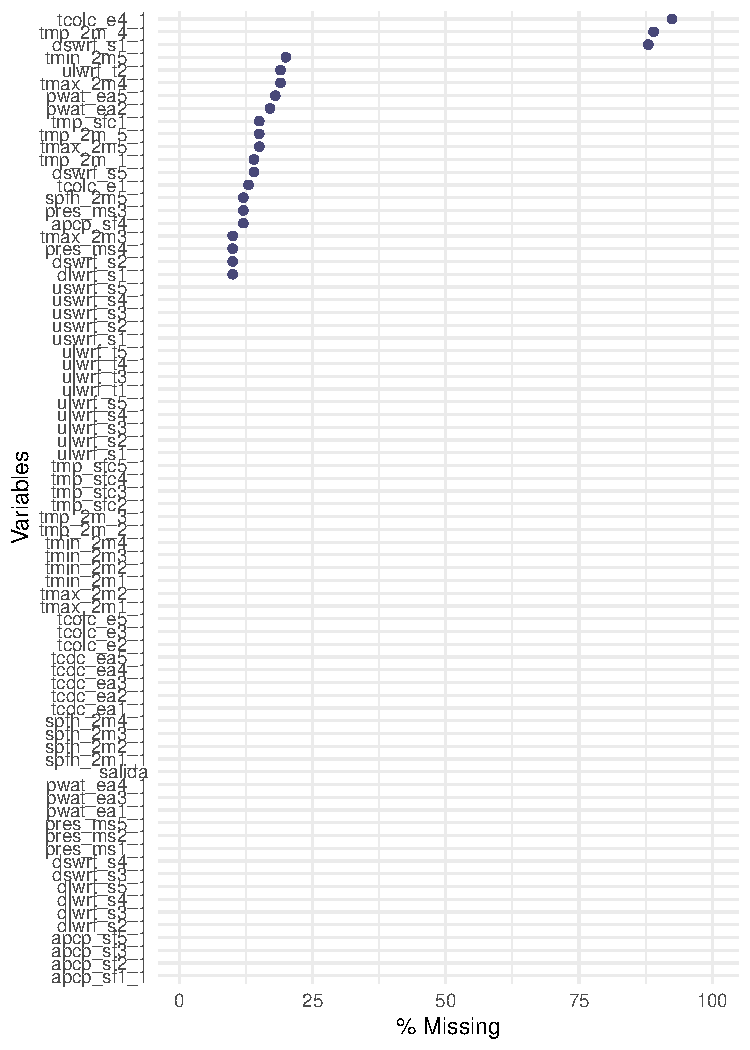
\includegraphics{memoria_practica_1_files/figure-latex/unnamed-chunk-4-1} \end{center}

Hay que diferenciar variables que toman valores constantes de aquellas
que toman valores muy pequeños, ya que en ambos casos la desviación
típica es igual o muy próxima a 0, estas son: \texttt{dswrf\_s1\_1},
\texttt{dswrf\_s2\_1}, \texttt{spfh\_2m1\_1}, \texttt{spfh\_2m5\_1},
\texttt{tcdc\_ea5\_1}, \texttt{tcolc\_e1\_1}, \texttt{tcolc\_e4\_1},
\texttt{tmp\_sfc1\_1} y \texttt{uswrf\_s2\_1}.

\begin{Shaded}
\begin{Highlighting}[]
\NormalTok{(variables\_numericas\_poca\_variabilidad }\OtherTok{\textless{}{-}}\NormalTok{ skim\_exploratorio }\SpecialCharTok{\%\textgreater{}\%} \FunctionTok{filter}\NormalTok{(skim\_type }\SpecialCharTok{==} \StringTok{"numeric"} \SpecialCharTok{\&}\NormalTok{ numeric.sd }\SpecialCharTok{\textless{}} \DecValTok{1}\NormalTok{) }\SpecialCharTok{\%\textgreater{}\%} \FunctionTok{select}\NormalTok{(skim\_variable) }\SpecialCharTok{\%\textgreater{}\%} \FunctionTok{as.data.frame}\NormalTok{() }\SpecialCharTok{\%\textgreater{}\%} \FunctionTok{as.matrix}\NormalTok{() }\SpecialCharTok{\%\textgreater{}\%} \FunctionTok{as.vector}\NormalTok{())}
\end{Highlighting}
\end{Shaded}

\begin{verbatim}
## [1] "dswrf_s1_1" "spfh_2m1_1" "spfh_2m5_1" "tcdc_ea5_1" "tcolc_e1_1"
## [6] "tcolc_e4_1" "tmp_sfc1_1" "uswrf_s2_1"
\end{verbatim}

Vamos a ver si realmente son constantes o solamente es que toman valores
muy pequeños y por ello la desviación típica tiende a cero. Para ello
nos basaremos en los histogramas:

\begin{Shaded}
\begin{Highlighting}[]
\ControlFlowTok{for}\NormalTok{(i }\ControlFlowTok{in}\NormalTok{ variables\_numericas\_poca\_variabilidad)\{}
\NormalTok{        datos\_disp }\SpecialCharTok{\%\textgreater{}\%} \FunctionTok{select}\NormalTok{(i) }\SpecialCharTok{\%\textgreater{}\%} \FunctionTok{as.matrix}\NormalTok{() }\SpecialCharTok{\%\textgreater{}\%} \FunctionTok{as.vector}\NormalTok{() }\SpecialCharTok{\%\textgreater{}\%} \FunctionTok{na.omit}\NormalTok{() }\SpecialCharTok{\%\textgreater{}\%} \FunctionTok{hist}\NormalTok{(}\AttributeTok{main =}\NormalTok{ i)}
\NormalTok{\}}
\end{Highlighting}
\end{Shaded}

\begin{verbatim}
## Warning: Using an external vector in selections was deprecated in tidyselect 1.1.0.
## i Please use `all_of()` or `any_of()` instead.
##   # Was:
##   data %>% select(i)
## 
##   # Now:
##   data %>% select(all_of(i))
## 
## See <https://tidyselect.r-lib.org/reference/faq-external-vector.html>.
\end{verbatim}

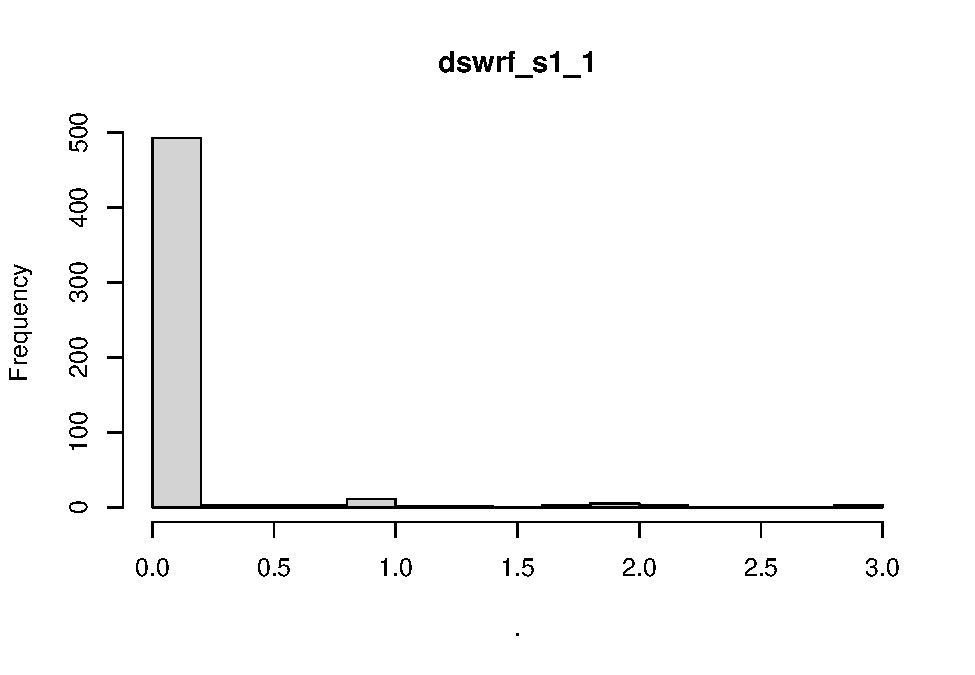
\includegraphics{memoria_practica_1_files/figure-latex/unnamed-chunk-6-1.pdf}
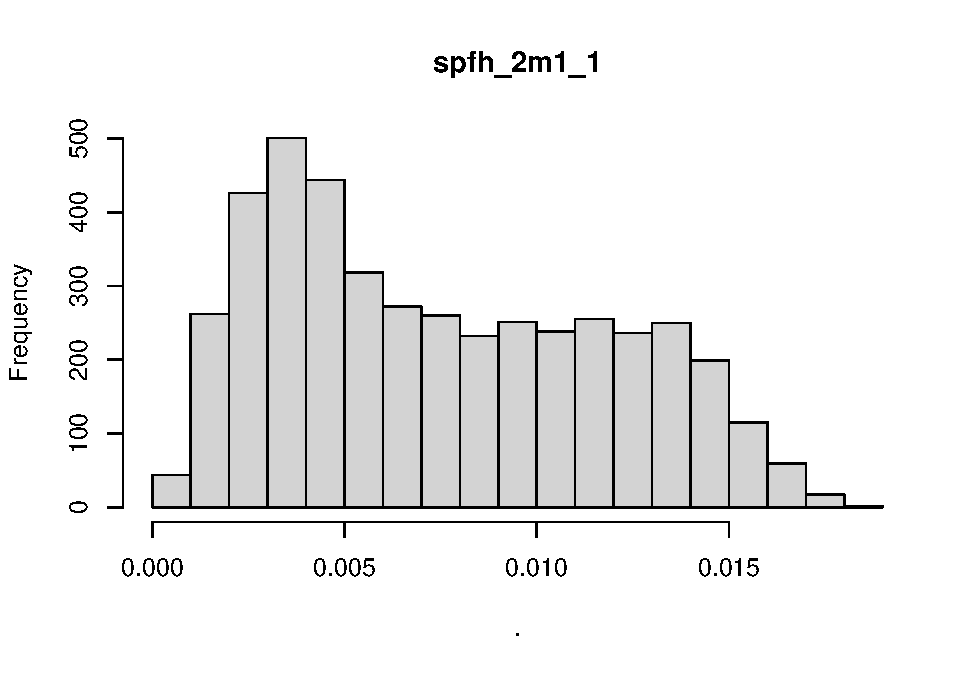
\includegraphics{memoria_practica_1_files/figure-latex/unnamed-chunk-6-2.pdf}
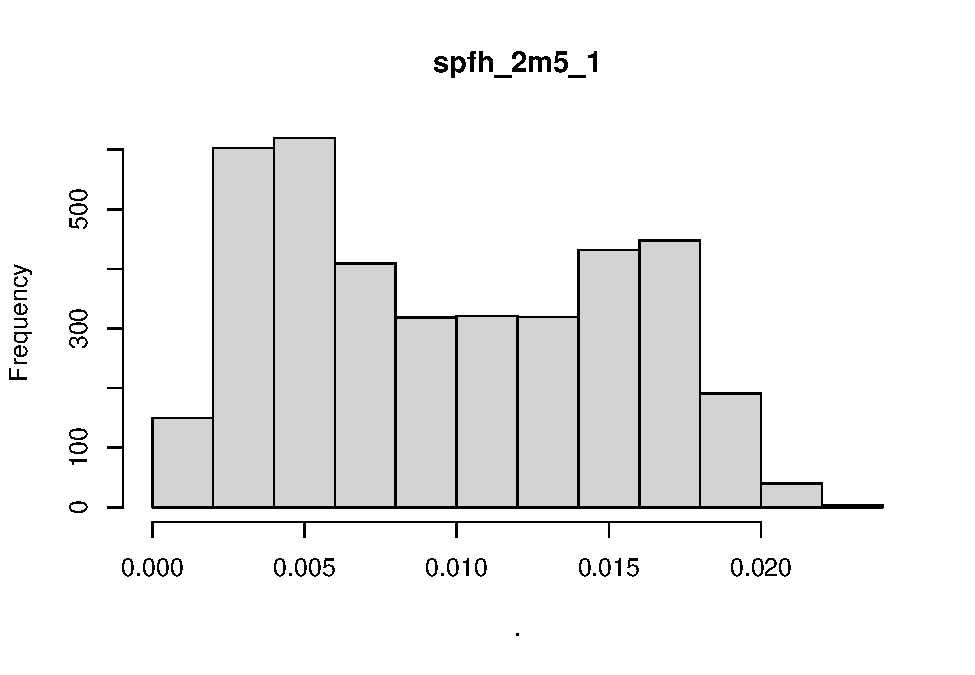
\includegraphics{memoria_practica_1_files/figure-latex/unnamed-chunk-6-3.pdf}
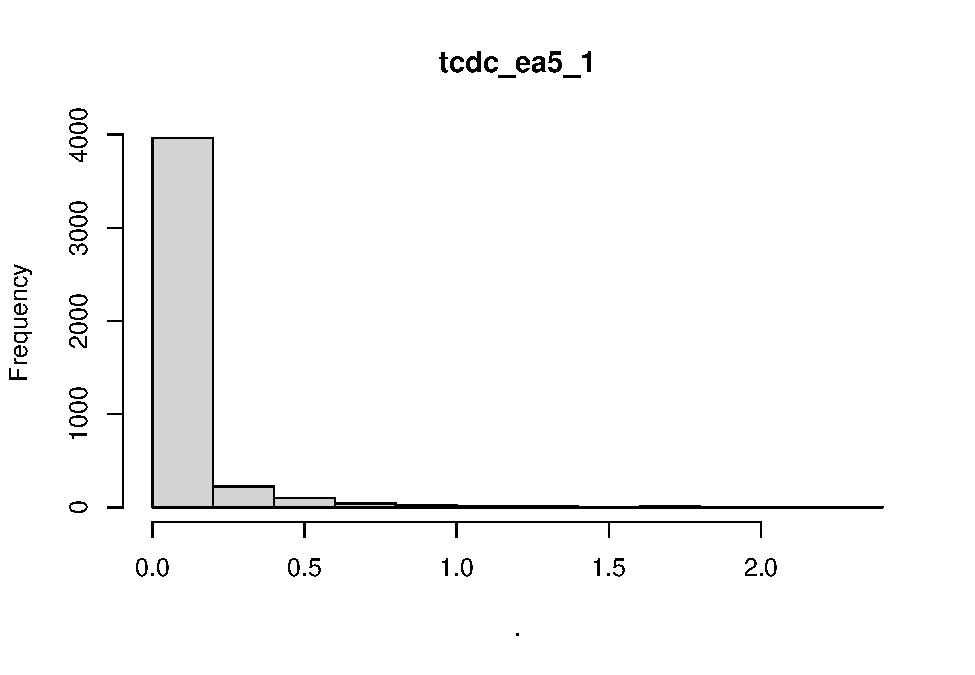
\includegraphics{memoria_practica_1_files/figure-latex/unnamed-chunk-6-4.pdf}
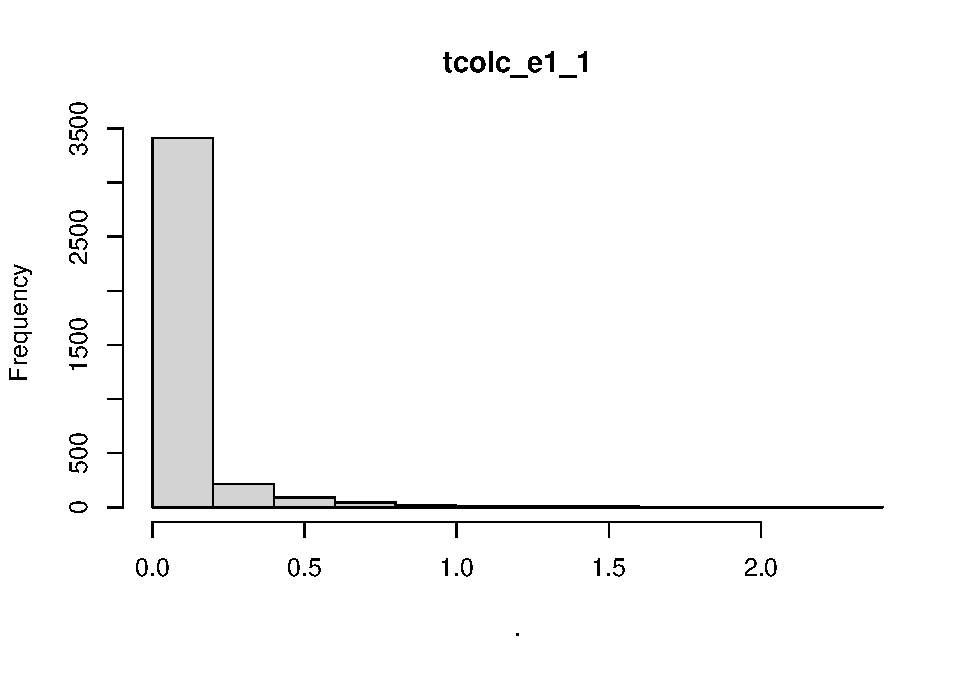
\includegraphics{memoria_practica_1_files/figure-latex/unnamed-chunk-6-5.pdf}
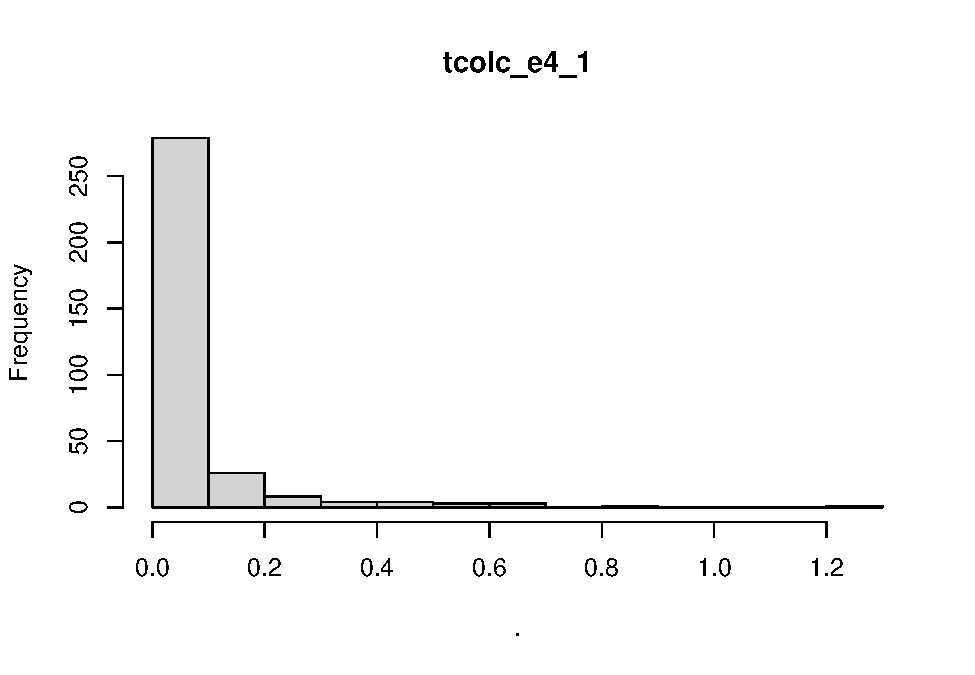
\includegraphics{memoria_practica_1_files/figure-latex/unnamed-chunk-6-6.pdf}
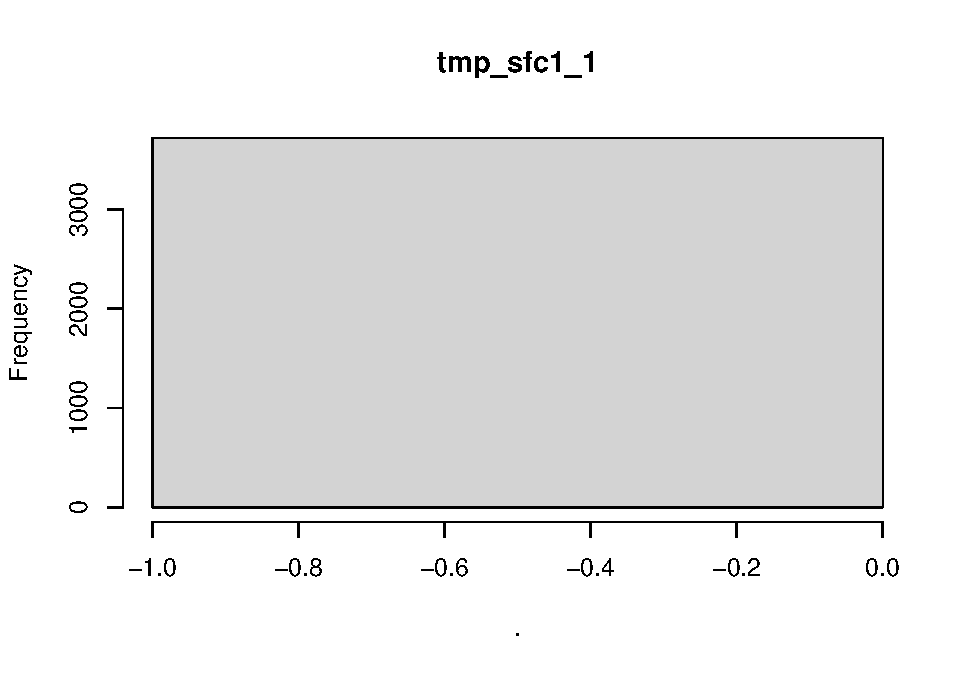
\includegraphics{memoria_practica_1_files/figure-latex/unnamed-chunk-6-7.pdf}
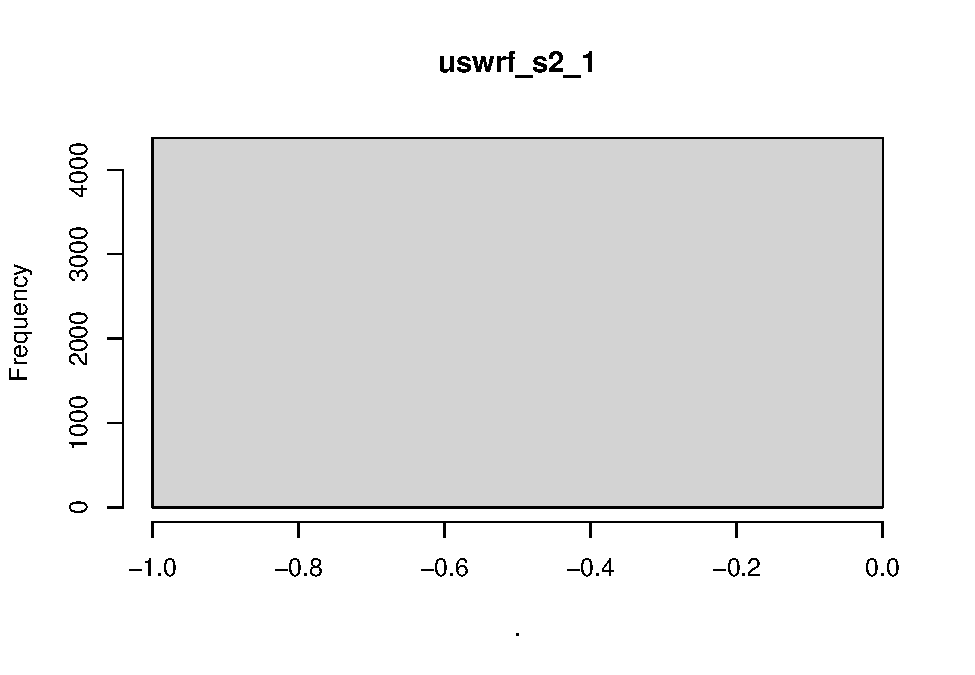
\includegraphics{memoria_practica_1_files/figure-latex/unnamed-chunk-6-8.pdf}

Podemos ver que las variables \texttt{dswrf\_s1\_1},
\texttt{tcdc\_ea5\_1}, \texttt{tcolc\_e1\_1}, \texttt{tcolc\_e4\_1},
\texttt{tmp\_sfc1\_1} y \texttt{uswrf\_s2\_1} son efectivamente
constantes, mientras que \texttt{spfh\_2m1\_1} y \texttt{spfh\_2m5\_1}
tienen poca variabilidad por tener valores muy pequeños, pero sí tienen
variabilidad. Con lo que guardamos dichas variables para posteriores
acciones:

\begin{Shaded}
\begin{Highlighting}[]
\NormalTok{variables\_numericas\_constantes }\OtherTok{\textless{}{-}} \FunctionTok{c}\NormalTok{(}\StringTok{"dswrf\_s1\_1"}\NormalTok{, }\StringTok{"tcdc\_ea5\_1"}\NormalTok{, }\StringTok{"tcolc\_e1\_1"}\NormalTok{, }\StringTok{"tcolc\_e4\_1"}\NormalTok{, }\StringTok{"tmp\_sfc1\_1"}\NormalTok{, }\StringTok{"uswrf\_s2\_1"}\NormalTok{)}
\end{Highlighting}
\end{Shaded}

Convertiremos todos los datos que no sean numéricos en \texttt{factor},
especialmente los \texttt{character}, que pueden dar problemas en
futuras aplicaciones:

\begin{Shaded}
\begin{Highlighting}[]
\NormalTok{variables\_character }\OtherTok{\textless{}{-}}\NormalTok{ skim\_exploratorio }\SpecialCharTok{\%\textgreater{}\%} \FunctionTok{filter}\NormalTok{(skim\_type }\SpecialCharTok{==} \StringTok{"character"}\NormalTok{) }\SpecialCharTok{\%\textgreater{}\%} \FunctionTok{select}\NormalTok{(skim\_variable) }\SpecialCharTok{\%\textgreater{}\%} \FunctionTok{as.matrix}\NormalTok{() }\SpecialCharTok{\%\textgreater{}\%} \FunctionTok{as.vector}\NormalTok{()}
\NormalTok{datos\_disp[, variables\_character[}\DecValTok{1}\NormalTok{]] }\OtherTok{\textless{}{-}} \FunctionTok{as.factor}\NormalTok{(datos\_disp[, variables\_character[}\DecValTok{1}\NormalTok{]])}
\NormalTok{datos\_disp[, variables\_character[}\DecValTok{2}\NormalTok{]] }\OtherTok{\textless{}{-}} \FunctionTok{as.factor}\NormalTok{(datos\_disp[, variables\_character[}\DecValTok{2}\NormalTok{]])}
\NormalTok{practica\_1\_task }\OtherTok{\textless{}{-}} \FunctionTok{as\_task\_regr}\NormalTok{(datos\_disp, }\AttributeTok{target =} \StringTok{"salida"}\NormalTok{, }\AttributeTok{id =} \StringTok{"radiacion"}\NormalTok{)}
\end{Highlighting}
\end{Shaded}

\subsection{Variable respuesta}

A continuación graficaremos la variable respuesta en el tiempo:

\begin{Shaded}
\begin{Highlighting}[]
\NormalTok{vector\_indicador }\OtherTok{\textless{}{-}} \DecValTok{1}\SpecialCharTok{:}\FunctionTok{nrow}\NormalTok{(datos\_disp)}
\NormalTok{datos\_grafico\_respuesta }\OtherTok{\textless{}{-}} \FunctionTok{data.frame}\NormalTok{(}\AttributeTok{indice =}\NormalTok{ vector\_indicador, }\AttributeTok{salida =}\NormalTok{ datos\_disp}\SpecialCharTok{$}\NormalTok{salida) }
\FunctionTok{ggplot}\NormalTok{(}\AttributeTok{data =}\NormalTok{ datos\_grafico\_respuesta, }\FunctionTok{aes}\NormalTok{(}\AttributeTok{x =}\NormalTok{ vector\_indicador, }\AttributeTok{y =}\NormalTok{ salida)) }\SpecialCharTok{+} \FunctionTok{geom\_line}\NormalTok{() }\SpecialCharTok{+} \FunctionTok{xlab}\NormalTok{(}\StringTok{"día"}\NormalTok{) }\SpecialCharTok{+} \FunctionTok{ylab}\NormalTok{(}\StringTok{"salida"}\NormalTok{) }\SpecialCharTok{+} \FunctionTok{ggtitle}\NormalTok{(}\StringTok{"Radiación a lo largo del tiempo (1996{-}2008)"}\NormalTok{)}
\end{Highlighting}
\end{Shaded}

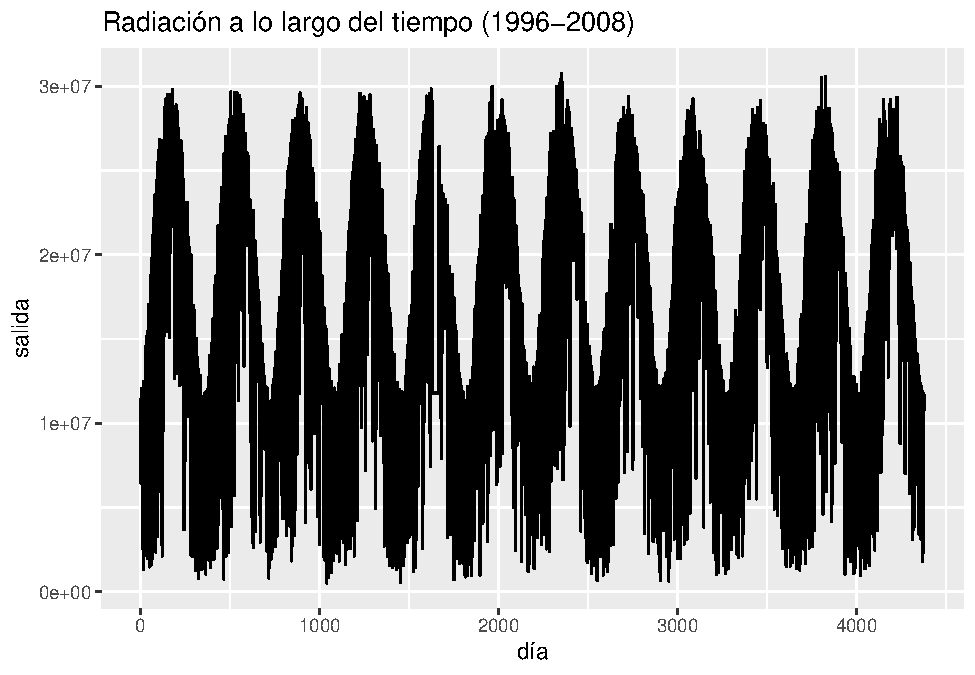
\includegraphics{memoria_practica_1_files/figure-latex/unnamed-chunk-9-1.pdf}

Podemos ver que existe una clara estacionalidad en la radiación captada
por las placas solares, aunque el nivel de la serie parece constante en
el tiempo, es decir, no se observan tendencias crecientes ni
decrecientes en los datos, esto es, los niveles de radiación son
parecidos año tras año.

\section{Métrica: Relative Absolute Error}

El error absoluto relativo (RAE en inglés) para un modelo de regresión
con variable respuesta \(y_i\) puede ser definido como: \[
RAE(\hat{y_i}) = \frac{\sum_{i=1}^n |y_i - \hat{y_i}|}{\sum_{i=1}^n |y_i - \overline{y}|}
\] dónde \(\hat{y_i}\) es la predicción de la variable respuesta que
hace el modelo de regresión e
\(\overline{y} = \frac{1}{n}\sum_{i=1}^n y_i\). Se puede interpretar
como un ratio entre el error absoluto de predicción con el modelo
escogido y el error absoluto para una predicción \emph{naive} basada en
la media de la respuesta \(\overline{y}\). Esta medida no está definida
para el caso \(y_i = y \quad \forall i=1, \dots, n\).

Este ratio puede ser usado mediante la librería \texttt{mlr3} mediante
instanciado a través del diccionario \texttt{mlr\_measures} o mediante
la función asociada \texttt{msr()}:

\begin{Shaded}
\begin{Highlighting}[]
\NormalTok{mlr\_measures}\SpecialCharTok{$}\FunctionTok{get}\NormalTok{(}\StringTok{"regr.rae"}\NormalTok{)}
\NormalTok{(measure }\OtherTok{\textless{}{-}} \FunctionTok{msr}\NormalTok{(}\StringTok{"regr.rae"}\NormalTok{))}
\end{Highlighting}
\end{Shaded}

\newpage
\section{Mejor método de imputación y de escalado}

En este apartado vamos a comparar distintos métodos de imputación y
escalado en base a su RAE en el conjunto de testeo para un modelo de
vecino más cercano con hiper-parámetros por defecto.

\subsection{Eliminación de las variables que toman valores constantes y/o tienen muchos NA}

Eliminaremos del modelo aquellos predictores que tienen valores
constante o varianzas muy próximas a cero y también aquellos que tienen
un porcentaje de NA muy elevado (véase Análisis Exploratorio de Datos):

\begin{Shaded}
\begin{Highlighting}[]
\NormalTok{datos\_disp }\OtherTok{\textless{}{-}}\NormalTok{ datos\_disp }\SpecialCharTok{\%\textgreater{}\%} \FunctionTok{select}\NormalTok{(}\SpecialCharTok{{-}}\NormalTok{(}\FunctionTok{all\_of}\NormalTok{(}\FunctionTok{c}\NormalTok{(variables\_numericas\_constantes, variables\_numericas\_muchos\_NA))))}
\NormalTok{datos\_compet }\OtherTok{\textless{}{-}}\NormalTok{ datos\_compet }\SpecialCharTok{\%\textgreater{}\%} \FunctionTok{select}\NormalTok{(}\SpecialCharTok{{-}}\NormalTok{(}\FunctionTok{all\_of}\NormalTok{(}\FunctionTok{c}\NormalTok{(variables\_numericas\_constantes, variables\_numericas\_muchos\_NA))))}
\NormalTok{practica\_1\_task }\OtherTok{\textless{}{-}} \FunctionTok{as\_task\_regr}\NormalTok{(datos\_disp, }\AttributeTok{target =} \StringTok{"salida"}\NormalTok{, }\AttributeTok{id =} \StringTok{"radiacion"}\NormalTok{)}
\end{Highlighting}
\end{Shaded}

\subsection{Particiones de entrenamiento y test}

A continuación dividiremos el conjunto de datos \texttt{datos\_disp} en
particiones de entrenamiento y testeo, correspondiendo los datos de los
primeros 9 años a datos de entrenamiento, y los 3 últimos años a
validación:

\begin{Shaded}
\begin{Highlighting}[]
\FunctionTok{set.seed}\NormalTok{(}\DecValTok{100430509}\NormalTok{) }\CommentTok{\# NIA de Marc Pastor}
\CommentTok{\#source("./info/Ajuste Hiper{-}parámetros/ResamplingHoldoutOrder.R")}
\CommentTok{\#desc\_inner \textless{}{-} rsmp("holdoutorder", ratio = 6/9)}
\NormalTok{desc\_outer }\OtherTok{\textless{}{-}} \FunctionTok{rsmp}\NormalTok{(}\StringTok{"custom"}\NormalTok{)}
\NormalTok{desc\_outer}\SpecialCharTok{$}\FunctionTok{instantiate}\NormalTok{(practica\_1\_task, }
                       \AttributeTok{train =} \FunctionTok{list}\NormalTok{(}\DecValTok{1}\SpecialCharTok{:}\NormalTok{(}\DecValTok{9}\SpecialCharTok{*}\DecValTok{365}\NormalTok{)),}
                       \AttributeTok{test =} \FunctionTok{list}\NormalTok{((}\DecValTok{9}\SpecialCharTok{*}\DecValTok{365}\SpecialCharTok{+}\DecValTok{1}\NormalTok{)}\SpecialCharTok{:}\NormalTok{(}\DecValTok{12}\SpecialCharTok{*}\DecValTok{365}\NormalTok{)))}
\end{Highlighting}
\end{Shaded}

\subsection{Métodos de escalado}
\subsubsection{Normalización de los datos}

Eliminamos las constantes, normalizamos los datos y hacemos una
codificación \emph{one-hot} de las variables cualitativas:

\begin{Shaded}
\begin{Highlighting}[]
\NormalTok{preproc\_inicial }\OtherTok{\textless{}{-}} \FunctionTok{po}\NormalTok{(}\StringTok{"removeconstants"}\NormalTok{) }\SpecialCharTok{\%\textgreater{}\textgreater{}\%} \FunctionTok{po}\NormalTok{(}\StringTok{"encode"}\NormalTok{)}
\NormalTok{practica\_1\_task }\OtherTok{\textless{}{-}}\NormalTok{ preproc\_inicial}\SpecialCharTok{$}\FunctionTok{train}\NormalTok{(practica\_1\_task)[[}\DecValTok{1}\NormalTok{]]}

\NormalTok{id\_train }\OtherTok{\textless{}{-}}\NormalTok{ desc\_outer}\SpecialCharTok{$}\FunctionTok{train\_set}\NormalTok{(}\AttributeTok{i =} \DecValTok{1}\NormalTok{)}
\NormalTok{id\_test }\OtherTok{\textless{}{-}}\NormalTok{ desc\_outer}\SpecialCharTok{$}\FunctionTok{test\_set}\NormalTok{(}\AttributeTok{i =} \DecValTok{1}\NormalTok{)}

\CommentTok{\# Se crean dos nuevas task, una con los datos de train y otra con los de test.}
\CommentTok{\# Dado que se va a aplicar un filtrado, y para no alterar task\_datos, se emplea}
\CommentTok{\# antes del filtro el método $clone() para hacer una copia.}
\NormalTok{task\_train }\OtherTok{\textless{}{-}}\NormalTok{ practica\_1\_task}\SpecialCharTok{$}\FunctionTok{clone}\NormalTok{()}\SpecialCharTok{$}\FunctionTok{filter}\NormalTok{(id\_train)}
\NormalTok{task\_test  }\OtherTok{\textless{}{-}}\NormalTok{ practica\_1\_task}\SpecialCharTok{$}\FunctionTok{clone}\NormalTok{()}\SpecialCharTok{$}\FunctionTok{filter}\NormalTok{(id\_test)}
\end{Highlighting}
\end{Shaded}

\subsection{Métodos de imputación multivariante}

En esta sección usaremos distintos métodos de imputación multivariante
ya que disponemos de datos multivariantes, tanto variables continuas,
como categóricas, etc.

\subsubsection{Imputación mediante AMELIA (\emph{Multiple Imputation of Incomplete Multivariate Data})}

AMELIA es un procedimiento para imputar datos multivariantes. Entre sus
supuestos el principal es asumir que los datos (tanto observados como
no) siguen una distribución normal multivariante. Si denotamos el
\emph{dataset} de tamaño \((n \times k)\) como \(D\), enconces esta
asunción es: \[
D \sim \mathcal{N}_k(\mu, \Sigma).
\]

En nuestro caso los datos no son solamente continuos, sino que hay
variables categóricas y discretas, por lo que esta asunción no se va a
dar. Por ello, descartaremos este procedimiento.

\subsubsection{MICE: \emph{Multiple Imputation by Chained Equations}}

MICE es un método de imputación múltiple que se basa en el supuesto de
que dadas las variables usadas en el proceso de imputación, los datos
faltantes son MAR (\emph{Missing At Random}), lo cuál significa que la
probabilidad de que un valor sea faltante depende solo de los valores
observados y no de los valores que no han sido observados. En otras
palabras, después de controlar todos los datos disponibles (es decir,
las variables incluidas en el modelo de imputación), cualquier dato
faltante es completamente aleatorio. Implementar MICE cuando los datos
no son MAR podría dar lugar a estimaciones sesgadas. De aquí en
adelante, supondremos que nuestros datos son MAR.

Muchos de los modelos de imputación múltiples inicialmente
desarrollados, asumen una distribución conjunta de todas las variables,
por ejemplo la distribución normal, lo cuál no suele ocurrir en
conjuntos de datos grandes, con decenas de variables de distintos tipos.
MICE ofrece una alternativa flexible basada en modelos de regresión
donde los datos faltantes se modelan en función de las variables
disponibles en los datos. Esto implica que cada variable puede ser
modelada en base a su distribución, por ejemplo las variables binarias
con regresión logística y las continuas con regresión lineal, etc.

\textbf{Procedimiento MICE}

El algoritmo MICE puede ser dividido en 4 grandes pasos:

\begin{enumerate}
\item Se ejecuta una imputación simple, por ejemplo imputación mediante la media, para cada valor faltante en el \emph{dataset}. Estas imputaciones sencillas pueden ser pensadas como imputaciones base. 
\item Las imputaciones base para cada variable $X_i$ vuelven a ser asignadas el valor de faltante/missing.
\item Los valores observados de la variable $X_i$ en el paso 2 se modelan como un modelo de regresión en función del resto de variables en el \emph{dataset}. Estos modelos de regresión operan bajo los supuestos que uno haria cuando realiza regresión logística, lineal o Poisson fuera del contexto de datos faltantes.
\item Los valores faltantes de la variable $X_i$ son reemplazados por las predicciones (imputaciones) del modelo de regresión. Cuando $X_i$ posteriormente se utilice en los modelos de regresión para otras variables, se utilizarán tanto los valores observados como los imputados.
\item Se repiten los pasos 2-4 para cada variable que tiene datos faltantes. El proceso para cada una de las variables constituye una iteración o ciclo. Al final de cada ciclo, todos los valores faltantes han sido sustituidos por predicciones de regresiones que representan las relaciones entre los datos observados. 
\item Los pasos 2-4 se repiten para un número de ciclos, con las imputaciones siendo actualizadas en cada ciclo.
\end{enumerate}

El número de ciclos a realizarse puede ser escogido por el investigador,
aunque generalmente se llevan a cabo 10. La idea es que al final de los
ciclos, la distribución de los parámetros que gobiernan las imputaciones
(por ejemplo los coeficientes de los modelos de regresión) deben haber
convergido, en el sentido de volverse estables.

\begin{Shaded}
\begin{Highlighting}[]
\NormalTok{imp }\OtherTok{\textless{}{-}}\NormalTok{ PipeOpMice}\SpecialCharTok{$}\FunctionTok{new}\NormalTok{()}
\CommentTok{\# learner }
\NormalTok{learner }\OtherTok{\textless{}{-}} \FunctionTok{lrn}\NormalTok{(}\StringTok{\textquotesingle{}regr.kknn\textquotesingle{}}\NormalTok{)}

\NormalTok{graph }\OtherTok{\textless{}{-}}\NormalTok{ imp }\SpecialCharTok{\%\textgreater{}\textgreater{}\%} \FunctionTok{po}\NormalTok{(learner)}

\NormalTok{graph\_learner }\OtherTok{\textless{}{-}}\NormalTok{ GraphLearner}\SpecialCharTok{$}\FunctionTok{new}\NormalTok{(graph, }\AttributeTok{id =} \StringTok{\textquotesingle{}mice.learner\textquotesingle{}}\NormalTok{)}
\NormalTok{graph\_learner}\SpecialCharTok{$}\NormalTok{id }\OtherTok{\textless{}{-}}  \StringTok{\textquotesingle{}mice.learner\textquotesingle{}}
\CommentTok{\# resampling }
\FunctionTok{set.seed}\NormalTok{(}\DecValTok{100430509}\NormalTok{)}
\NormalTok{knn\_resample }\OtherTok{\textless{}{-}} \FunctionTok{resample}\NormalTok{(practica\_1\_task, graph\_learner, desc\_outer)}
\end{Highlighting}
\end{Shaded}

\begin{verbatim}
## INFO  [17:11:28.399] [mlr3] Applying learner 'mice.learner' on task 'radiacion' (iter 1/1)
\end{verbatim}

\begin{verbatim}
## Error in value[[3L]](cond): Error in solve.default(xtx + diag(pen)): sistema es computacionalmente singular: número de condición recíproco = 7.4371e-17
## 
## This happened PipeOp impute_mice_B's $train()
\end{verbatim}

\begin{Shaded}
\begin{Highlighting}[]
\NormalTok{knn\_rae }\OtherTok{\textless{}{-}}\NormalTok{ knn\_resample}\SpecialCharTok{$}\FunctionTok{aggregate}\NormalTok{(}\FunctionTok{msr}\NormalTok{(}\StringTok{"regr.rae"}\NormalTok{))}
\end{Highlighting}
\end{Shaded}

\begin{verbatim}
## Error in eval(expr, envir, enclos): objeto 'knn_resample' no encontrado
\end{verbatim}

\begin{Shaded}
\begin{Highlighting}[]
\FunctionTok{print}\NormalTok{(knn\_rae)}
\end{Highlighting}
\end{Shaded}

\begin{verbatim}
## Error in print(knn_rae): objeto 'knn_rae' no encontrado
\end{verbatim}

Parece que uno de los sistemas de ecuaciones es singular, por lo que el
programa no encuentra solución, y por ello el algoritmo no nos es útil.

\subsubsection{missForest}

Se trata de un procedimiento que \emph{random forest} para predecir el
valor de los datos faltantes:

\begin{Shaded}
\begin{Highlighting}[]
\NormalTok{imp }\OtherTok{\textless{}{-}}\NormalTok{ PipeOpmissForest}\SpecialCharTok{$}\FunctionTok{new}\NormalTok{()}
\CommentTok{\# learner }
\NormalTok{learner }\OtherTok{\textless{}{-}} \FunctionTok{lrn}\NormalTok{(}\StringTok{\textquotesingle{}regr.kknn\textquotesingle{}}\NormalTok{)}

\NormalTok{graph }\OtherTok{\textless{}{-}}\NormalTok{ imp }\SpecialCharTok{\%\textgreater{}\textgreater{}\%}\NormalTok{  learner}

\NormalTok{graph\_learner }\OtherTok{\textless{}{-}}\NormalTok{ GraphLearner}\SpecialCharTok{$}\FunctionTok{new}\NormalTok{(graph, }\AttributeTok{id =} \StringTok{\textquotesingle{}missForest.learner\textquotesingle{}}\NormalTok{)}
\NormalTok{graph\_learner}\SpecialCharTok{$}\NormalTok{id }\OtherTok{\textless{}{-}}  \StringTok{\textquotesingle{}missForest.learner\textquotesingle{}}
\CommentTok{\# resampling }
\FunctionTok{set.seed}\NormalTok{(}\DecValTok{100430509}\NormalTok{)}
\NormalTok{knn\_resample }\OtherTok{\textless{}{-}} \FunctionTok{resample}\NormalTok{(practica\_1\_task, graph\_learner, desc\_outer)}
\end{Highlighting}
\end{Shaded}

\begin{verbatim}
## INFO  [17:11:54.804] [mlr3] Applying learner 'missForest.learner' on task 'radiacion' (iter 1/1)
\end{verbatim}

\begin{Shaded}
\begin{Highlighting}[]
\NormalTok{knn\_rae }\OtherTok{\textless{}{-}}\NormalTok{ knn\_resample}\SpecialCharTok{$}\FunctionTok{aggregate}\NormalTok{(}\FunctionTok{msr}\NormalTok{(}\StringTok{"regr.rae"}\NormalTok{))}
\FunctionTok{print}\NormalTok{(knn\_rae)}
\end{Highlighting}
\end{Shaded}

\begin{verbatim}
##  regr.rae 
## 0.4343481
\end{verbatim}

\subsubsection{Miss Ranger}

Utilizaremos el algoritmo \texttt{MissRanger}, que es una versión
mejorada de \texttt{MissForest} en la que se añade el emparejamiento
predictivo de medias entre iteraciones de los random forest. Esto evita
en primer lugar imputación con valores que no estén presentes en los
datos y en segundo lugar, el emparejamiento predictivo de medias intenta
incrementar la varianza de las distribuciones condicionales para
alcanzar un nivel realista.

\begin{Shaded}
\begin{Highlighting}[]
\NormalTok{imp }\OtherTok{\textless{}{-}}\NormalTok{ PipeOpmissRanger}\SpecialCharTok{$}\FunctionTok{new}\NormalTok{()}
\CommentTok{\# learner }
\NormalTok{learner }\OtherTok{\textless{}{-}} \FunctionTok{lrn}\NormalTok{(}\StringTok{\textquotesingle{}regr.kknn\textquotesingle{}}\NormalTok{)}

\NormalTok{graph }\OtherTok{\textless{}{-}}\NormalTok{ imp }\SpecialCharTok{\%\textgreater{}\textgreater{}\%}\NormalTok{ learner}

\NormalTok{graph\_learner }\OtherTok{\textless{}{-}}\NormalTok{ GraphLearner}\SpecialCharTok{$}\FunctionTok{new}\NormalTok{(graph, }\AttributeTok{id =} \StringTok{\textquotesingle{}missRanger.learner\textquotesingle{}}\NormalTok{)}
\NormalTok{graph\_learner}\SpecialCharTok{$}\NormalTok{id }\OtherTok{\textless{}{-}}  \StringTok{\textquotesingle{}missRanger.learner\textquotesingle{}}
\CommentTok{\# resampling }
\FunctionTok{set.seed}\NormalTok{(}\DecValTok{100430509}\NormalTok{)}
\NormalTok{knn\_resample }\OtherTok{\textless{}{-}} \FunctionTok{resample}\NormalTok{(practica\_1\_task, graph\_learner, desc\_outer)}
\end{Highlighting}
\end{Shaded}

\begin{verbatim}
## INFO  [17:26:36.639] [mlr3] Applying learner 'missRanger.learner' on task 'radiacion' (iter 1/1)
\end{verbatim}

\begin{Shaded}
\begin{Highlighting}[]
\NormalTok{knn\_rae }\OtherTok{\textless{}{-}}\NormalTok{ knn\_resample}\SpecialCharTok{$}\FunctionTok{aggregate}\NormalTok{(}\FunctionTok{msr}\NormalTok{(}\StringTok{"regr.rae"}\NormalTok{))}
\FunctionTok{print}\NormalTok{(knn\_rae)}
\end{Highlighting}
\end{Shaded}

\begin{verbatim}
##  regr.rae 
## 0.4399763
\end{verbatim}

Ahora que hemos visto que el método \emph{MissRanger} es el que menos
\texttt{rae} tiene de los que hemos probado, vamos a extraer los datos
de imputados y usarlos para crear una nueva \emph{task} con ellos.

\begin{Shaded}
\begin{Highlighting}[]
\NormalTok{graph\_learner\_missRanger\_trained }\OtherTok{\textless{}{-}}\NormalTok{ graph\_learner}\SpecialCharTok{$}\FunctionTok{train}\NormalTok{(practica\_1\_task)}
\NormalTok{datos\_imputados }\OtherTok{\textless{}{-}}\NormalTok{ graph\_learner\_missRanger\_trained}\SpecialCharTok{$}\NormalTok{graph\_model}\SpecialCharTok{$}\NormalTok{pipeops}\SpecialCharTok{$}\NormalTok{regr.kknn}\SpecialCharTok{$}\NormalTok{learner\_model}\SpecialCharTok{$}\NormalTok{model}
\NormalTok{datos\_imputados }\OtherTok{\textless{}{-}}\NormalTok{ datos\_imputados}\SpecialCharTok{$}\NormalTok{data}

\NormalTok{task\_DI }\OtherTok{\textless{}{-}}\NormalTok{ practica\_1\_task }\OtherTok{\textless{}{-}} \FunctionTok{as\_task\_regr}\NormalTok{(datos\_imputados, }\AttributeTok{target =} \StringTok{"salida"}\NormalTok{, }\AttributeTok{id =} \StringTok{"radiacion"}\NormalTok{)}
\NormalTok{task\_DI\_train }\OtherTok{\textless{}{-}}\NormalTok{ task\_DI}\SpecialCharTok{$}\FunctionTok{clone}\NormalTok{()}\SpecialCharTok{$}\FunctionTok{filter}\NormalTok{(id\_train)}
\NormalTok{task\_DI\_test  }\OtherTok{\textless{}{-}}\NormalTok{ task\_DI}\SpecialCharTok{$}\FunctionTok{clone}\NormalTok{()}\SpecialCharTok{$}\FunctionTok{filter}\NormalTok{(id\_test)}
\end{Highlighting}
\end{Shaded}

\section{Métodos para predecir}

En esta parte del trabajo vamos a probar con varios métodos para
predecir los datos de test, para luego ajustar hiperparámetros y ver si
ha mejorado, empeorado, o no han habido cambios en las predicciones.

\subsection{Sin ajuste de hiperparámetros}
\subsubsection{KNN}

Primero probaremos con el método de los K vecinos más cercanos, que
estima el valor de la función de probabiolidad de que un elemento
\(\mathcal{x}\) pertenezca a la clase \(\mathcal{C_j}\) a partir de la
información proporcionada por los predictores. Este es el caso de este
método para clasificación, pero aquí usaremos su versión para regresión,
que en lugar de establecer un sistema de votación considerando su clase,
se devuelve como predicción el valor medio de es clase.

Lo primero será crear el objeto learner para este modelo.

\begin{Shaded}
\begin{Highlighting}[]
\NormalTok{learner\_knn }\OtherTok{\textless{}{-}} \FunctionTok{lrn}\NormalTok{(}\StringTok{"regr.kknn"}\NormalTok{)}
\NormalTok{learner\_knn}\SpecialCharTok{$}\FunctionTok{train}\NormalTok{(}\AttributeTok{task =}\NormalTok{ task\_DI\_train)}

\NormalTok{knn\_predict }\OtherTok{\textless{}{-}}\NormalTok{ learner\_knn}\SpecialCharTok{$}\FunctionTok{predict}\NormalTok{(}\AttributeTok{task =}\NormalTok{ task\_DI\_test)}
\NormalTok{(knn\_rae }\OtherTok{\textless{}{-}}\NormalTok{ knn\_predict}\SpecialCharTok{$}\FunctionTok{score}\NormalTok{(measure))}
\end{Highlighting}
\end{Shaded}

\begin{verbatim}
##  regr.rae 
## 0.4360362
\end{verbatim}

Como podemos ver, el \textbf{Error Absouto Relativo (RAE)} para este
modelo sin ajustar hiperparámetros es de 0.436. Cuando los hayamos
ajustado todos veremos cuál es el que tiene menor RAE y, por lo tanto,
el mejor método para predecir sobre estos datos.

\subsubsection{Cubist}

Ahora vamos a probar con una regresión cubist, que se basa en hacer
árboles de regresión que tienen modelos de regresión lineal en las hojas
terminales que se basan en las predicciones hechas por los árboles que
les sirven para decidir cómo se va a dividir. En este caso no haremos
ajuste de hiperparámetros, por lo que voy a pasar directamente a crear
el learner para este modelo y hacer las predicciones en la muestra de
test.

\begin{Shaded}
\begin{Highlighting}[]
\NormalTok{learner\_cubist }\OtherTok{\textless{}{-}} \FunctionTok{lrn}\NormalTok{(}\StringTok{"regr.cubist"}\NormalTok{)}
\NormalTok{learner\_cubist}\SpecialCharTok{$}\FunctionTok{train}\NormalTok{(}\AttributeTok{task =}\NormalTok{ task\_DI\_train)}

\NormalTok{cubist\_predict }\OtherTok{\textless{}{-}}\NormalTok{ learner\_cubist}\SpecialCharTok{$}\FunctionTok{predict}\NormalTok{(}\AttributeTok{task =}\NormalTok{ task\_DI\_test)}
\NormalTok{(cubist\_rae }\OtherTok{\textless{}{-}}\NormalTok{ cubist\_predict}\SpecialCharTok{$}\FunctionTok{score}\NormalTok{(measure))}
\end{Highlighting}
\end{Shaded}

\begin{verbatim}
##  regr.rae 
## 0.3562076
\end{verbatim}

\subsubsection{rpart}

El siguiente método a probar será un arbol de regresión, que usa árboles
de decisión como modelo predictivo que mapea las observaciones de los
predictores. Este mapeado se hace al dividir las ramas en función de los
valores que toman los predictores para separarlos en hiper-rectángulos,
y la predicción de cualquier punto de un hiper-rectángulo será la media
de la variable salida de las observaciones que se encuentren en ese
hiper-rectángulo.

\begin{Shaded}
\begin{Highlighting}[]
\NormalTok{learner\_rpart }\OtherTok{\textless{}{-}} \FunctionTok{lrn}\NormalTok{(}\StringTok{"regr.rpart"}\NormalTok{)}
\NormalTok{learner\_rpart}\SpecialCharTok{$}\FunctionTok{train}\NormalTok{(}\AttributeTok{task =}\NormalTok{ task\_DI\_train)}

\NormalTok{rpart\_predict }\OtherTok{\textless{}{-}}\NormalTok{ learner\_rpart}\SpecialCharTok{$}\FunctionTok{predict}\NormalTok{(}\AttributeTok{task =}\NormalTok{ task\_DI\_test)}
\NormalTok{(rpart\_rae }\OtherTok{\textless{}{-}}\NormalTok{ rpart\_predict}\SpecialCharTok{$}\FunctionTok{score}\NormalTok{(measure))}
\end{Highlighting}
\end{Shaded}

\begin{verbatim}
##  regr.rae 
## 0.4721033
\end{verbatim}

\subsubsection{RandomForest}

También vamos a ajustar un random forest, que ajusta varios árboles de
regresión y crea una conmbinación de los mismos en función los valores
de una distribución aleatoria que es la misma para todos los árboles.

\begin{Shaded}
\begin{Highlighting}[]
\NormalTok{learner\_RF }\OtherTok{\textless{}{-}} \FunctionTok{lrn}\NormalTok{(}\StringTok{"regr.randomForest"}\NormalTok{)}
\NormalTok{learner\_RF}\SpecialCharTok{$}\FunctionTok{train}\NormalTok{(}\AttributeTok{task =}\NormalTok{ task\_DI\_train)}

\NormalTok{RF\_predict }\OtherTok{\textless{}{-}}\NormalTok{ learner\_RF}\SpecialCharTok{$}\FunctionTok{predict}\NormalTok{(}\AttributeTok{task =}\NormalTok{ task\_DI\_test)}
\NormalTok{(RF\_rae }\OtherTok{\textless{}{-}}\NormalTok{ RF\_predict}\SpecialCharTok{$}\FunctionTok{score}\NormalTok{(measure))}
\end{Highlighting}
\end{Shaded}

\begin{verbatim}
##  regr.rae 
## 0.3555573
\end{verbatim}

\subsubsection{Regresión Lineal Múltiple}

\emph{Esperar a parte de chiara}

\begin{Shaded}
\begin{Highlighting}[]
\NormalTok{learner\_lm }\OtherTok{\textless{}{-}} \FunctionTok{lrn}\NormalTok{(}\StringTok{"regr.lm"}\NormalTok{)}
\NormalTok{learner\_lm}\SpecialCharTok{$}\FunctionTok{train}\NormalTok{(}\AttributeTok{task =}\NormalTok{ task\_DI\_train)}

\NormalTok{lm\_predict }\OtherTok{\textless{}{-}}\NormalTok{ learner\_lm}\SpecialCharTok{$}\FunctionTok{predict}\NormalTok{(}\AttributeTok{task =}\NormalTok{ task\_DI\_test)}
\NormalTok{(lm\_rae }\OtherTok{\textless{}{-}}\NormalTok{ lm\_predict}\SpecialCharTok{$}\FunctionTok{score}\NormalTok{(measure))}
\end{Highlighting}
\end{Shaded}

\begin{verbatim}
##  regr.rae 
## 0.3573085
\end{verbatim}

\subsubsection{SVM}

Al ser un clasificador binario supervisado, la máquina de vectores de
soporte tiene el propósito de identificar un límite de separación
(lineal o de otro tipo) en un espacio de elementos de tal manera que las
observaciones posteriores se puedan clasificar automáticamente en grupos
separados. Este límite de separación puede ser una línea unidimensional,
como un plano o hiperplano, dependiendo de la dimensión en la que esté
trabajando. En este caso, en el que queremos predecir la radiación
solar, vamos a trabajar en un plano bidimensional.\\
Son posibles muchas fronteras de decisión y la frontera de decisión debe
estar tan lejos de ambas clases como sea posible, intentando de
maximizar el margin. Eso da lugar a la frontera con mejor capacidad de
generalización. La ubicación de los hiperplanos depende completamente de
la ubicación de los vectores de soporte. Al mover un vector de soporte,
el hiperplano se mueve de su ubicación original a una nueva ubicación.
El desplazamiento de un vector no compatible no tiene ningún impacto en
el hiperplano.\\
El algoritmo SVM puede aprender límites de decisión entre clases que no
son linealmente separables. Puede agregar otra dimensión a los datos,
para encontrar una forma lineal de separar los datos no lineales. La
dimensión extra se llama kernel (es decir, el producto escalar de los
vectores en el espacio transformado), se puede imaginar como un
``estiramiento'' de datos en una tercera dimensión. Esta dimensión
adicional le permite separar linealmente los datos. Cuando este
hiperplano se proyecta sobre las dos dimensiones originales, aparece
como un límite de decisión curvo. El algoritmo para encontrar el kernel
utiliza una transformación matemática de los datos llamada función
kernel, hay varias funciones del kernel y cada una de las cuales aplica
una transformación diferente a los datos y es adecuada para encontrar
límites de decisión lineales para diferentes situaciones:\\
\strut \\
- Kernel lineal\\
- Kernel polinómico\\
- Kernel radial, gausiano\\

Con el kernel lineal:

\begin{Shaded}
\begin{Highlighting}[]
\NormalTok{learner\_svm\_lin }\OtherTok{\textless{}{-}} \FunctionTok{lrn}\NormalTok{(}\StringTok{"regr.svm"}\NormalTok{, }\AttributeTok{kernel=}\StringTok{"linear"}\NormalTok{, }\AttributeTok{type=}\StringTok{"eps{-}regression"}\NormalTok{)}
\NormalTok{learner\_svm\_lin}\SpecialCharTok{$}\FunctionTok{train}\NormalTok{(}\AttributeTok{task =}\NormalTok{ task\_DI\_train)}
\NormalTok{svm\_lin\_predict }\OtherTok{\textless{}{-}}\NormalTok{ learner\_svm\_lin}\SpecialCharTok{$}\FunctionTok{predict}\NormalTok{(}\AttributeTok{task =}\NormalTok{ task\_DI\_test)}
\NormalTok{(svm\_lin\_rae }\OtherTok{\textless{}{-}}\NormalTok{ svm\_lin\_predict}\SpecialCharTok{$}\FunctionTok{score}\NormalTok{(measure))}
\end{Highlighting}
\end{Shaded}

\begin{verbatim}
##  regr.rae 
## 0.3434117
\end{verbatim}

Con el kernel radial:

\begin{Shaded}
\begin{Highlighting}[]
\NormalTok{learner\_svm\_rad }\OtherTok{\textless{}{-}} \FunctionTok{lrn}\NormalTok{(}\StringTok{"regr.svm"}\NormalTok{, }\AttributeTok{kernel=}\StringTok{"radial"}\NormalTok{, }\AttributeTok{type=}\StringTok{"eps{-}regression"}\NormalTok{)}
\NormalTok{learner\_svm\_rad}\SpecialCharTok{$}\FunctionTok{train}\NormalTok{(}\AttributeTok{task =}\NormalTok{ task\_DI\_train)}
\NormalTok{svm\_rad\_predict }\OtherTok{\textless{}{-}}\NormalTok{ learner\_svm\_rad}\SpecialCharTok{$}\FunctionTok{predict}\NormalTok{(}\AttributeTok{task =}\NormalTok{ task\_DI\_test)}
\NormalTok{(svm\_rad\_rae }\OtherTok{\textless{}{-}}\NormalTok{ svm\_rad\_predict}\SpecialCharTok{$}\FunctionTok{score}\NormalTok{(measure))}
\end{Highlighting}
\end{Shaded}

\begin{verbatim}
##  regr.rae 
## 0.3501929
\end{verbatim}

\subsubsection{Comparación}

Una vez ajustados todos los métodos sin ajuste de hiperparámetros, vamos
a ver cuál ha obtenido el menor RAE.

\begin{center}
\begin{tabular}{ |c|c|c|c|c|c|c| } 
\hline
\textbf{Ajuste hiper-par}           & \textbf{KNN}          & \textbf{Cubist}      &\textbf{rpart}      &\textbf{Randomforest}      &\textbf{Regresión}      &\textbf{SVM lineal}      &\textbf{SVM radial} \\
 \hline \hline 
 Sin & 0.4360362 & 0.3562076 & 0.4721033 & 0.3555573 & 0.3573085 & 0.3434117 & 0.3501929 
 \\
 \hline
\end{tabular}
\end{center}

Sin ajuste de hiperparámetros, el mejor modelo es el \emph{svm lineal},
con un \(RAE_{svm_lin} = 0.3434117\).

\subsection{Con ajuste de hiperparámetros}

Ahora ajustaremos los hiperparámetros de algunos de estos modelos para
ver si mejora su RAE y así poder elegir el mejor modelo de todos para
estos datos.

\subsubsection{KNN}

Para este modelo vamos a usar un grid search a la hora de hacer el
ajuste, que ajusta todos los modelos posibles dentro del espacio de
búsqueda, el cual decidiremos más adelante, y elige el que mejor
puntuación saque en la métrica seleccionada, en este caso el RAE.

Primero crearemos un desc\_inner sacado del archivo
\texttt{ResamplingHoldoutOrder.R}, ya que un custom resampling no
funciona con la función \texttt{Tuner}.

\begin{Shaded}
\begin{Highlighting}[]
\FunctionTok{source}\NormalTok{(}\StringTok{"ResamplingHoldoutOrder.R"}\NormalTok{)}
\NormalTok{desc\_inner }\OtherTok{\textless{}{-}} \FunctionTok{rsmp}\NormalTok{(}\StringTok{"holdoutorder"}\NormalTok{,}\AttributeTok{ratio=}\DecValTok{6}\SpecialCharTok{/}\DecValTok{9}\NormalTok{)}
\end{Highlighting}
\end{Shaded}

Una vez creado este resample, vamos a definir el espacio de búsqueda
para el grid search

\begin{Shaded}
\begin{Highlighting}[]
\NormalTok{knn\_space }\OtherTok{\textless{}{-}} \FunctionTok{ps}\NormalTok{(}\AttributeTok{k =} \FunctionTok{p\_int}\NormalTok{(}\AttributeTok{lower=}\DecValTok{1}\NormalTok{, }\AttributeTok{upper=}\DecValTok{20}\NormalTok{))}
\end{Highlighting}
\end{Shaded}

Con este espacio de búsqueda, el grid search ajustará todos los modelos
KNN con un número de vecinos entre 1 y 20. Una vez definido este espacio
de búsqueda ya podemos crear el learner para el ajuste de
hiperparámetros.

\begin{Shaded}
\begin{Highlighting}[]
\NormalTok{learner\_ajuste\_knn}\OtherTok{\textless{}{-}}\NormalTok{AutoTuner}\SpecialCharTok{$}\FunctionTok{new}\NormalTok{(}
  \AttributeTok{learner =}\NormalTok{ learner\_knn,}
  \AttributeTok{resampling =}\NormalTok{ desc\_inner,}
  \AttributeTok{measure =}\NormalTok{ measure,}
  \AttributeTok{search\_space =}\NormalTok{ knn\_space,}
  \AttributeTok{terminator =} \FunctionTok{trm}\NormalTok{(}\StringTok{"none"}\NormalTok{),}
  \AttributeTok{tuner=}\FunctionTok{tnr}\NormalTok{(}\StringTok{"grid\_search"}\NormalTok{),}
  \AttributeTok{store\_tuning\_instance =} \ConstantTok{TRUE}\NormalTok{)}

\CommentTok{\#Evaluamos el learner con auto ajuste}
\NormalTok{knn\_ajuste\_resample }\OtherTok{\textless{}{-}} \FunctionTok{resample}\NormalTok{(task\_DI,learner\_ajuste\_knn,desc\_outer,}\AttributeTok{store\_models =} \ConstantTok{TRUE}\NormalTok{)}
\end{Highlighting}
\end{Shaded}

\begin{verbatim}
## INFO  [17:30:22.240] [mlr3] Applying learner 'regr.kknn.tuned' on task 'radiacion' (iter 1/1)
## INFO  [17:30:22.284] [bbotk] Starting to optimize 1 parameter(s) with '<TunerGridSearch>' and '<TerminatorNone>'
## INFO  [17:30:22.288] [bbotk] Evaluating 1 configuration(s)
## INFO  [17:30:22.307] [mlr3] Running benchmark with 1 resampling iterations
## INFO  [17:30:22.314] [mlr3] Applying learner 'regr.kknn' on task 'radiacion' (iter 1/1)
## INFO  [17:30:22.615] [mlr3] Finished benchmark
## INFO  [17:30:22.653] [bbotk] Result of batch 1:
## INFO  [17:30:22.654] [bbotk]  k  regr.rae warnings errors runtime_learners
## INFO  [17:30:22.654] [bbotk]  1 0.5287437        0      0             0.27
## INFO  [17:30:22.654] [bbotk]                                 uhash
## INFO  [17:30:22.654] [bbotk]  67da1bf0-3794-4b35-8045-89f4bade17a8
## INFO  [17:30:22.656] [bbotk] Evaluating 1 configuration(s)
## INFO  [17:30:22.673] [mlr3] Running benchmark with 1 resampling iterations
## INFO  [17:30:22.680] [mlr3] Applying learner 'regr.kknn' on task 'radiacion' (iter 1/1)
## INFO  [17:30:23.046] [mlr3] Finished benchmark
## INFO  [17:30:23.083] [bbotk] Result of batch 2:
## INFO  [17:30:23.084] [bbotk]   k  regr.rae warnings errors runtime_learners
## INFO  [17:30:23.084] [bbotk]  16 0.4156899        0      0             0.35
## INFO  [17:30:23.084] [bbotk]                                 uhash
## INFO  [17:30:23.084] [bbotk]  1e8702fa-1b27-4380-aa40-fe962f559142
## INFO  [17:30:23.086] [bbotk] Evaluating 1 configuration(s)
## INFO  [17:30:23.102] [mlr3] Running benchmark with 1 resampling iterations
## INFO  [17:30:23.109] [mlr3] Applying learner 'regr.kknn' on task 'radiacion' (iter 1/1)
## INFO  [17:30:23.473] [mlr3] Finished benchmark
## INFO  [17:30:23.512] [bbotk] Result of batch 3:
## INFO  [17:30:23.514] [bbotk]   k  regr.rae warnings errors runtime_learners
## INFO  [17:30:23.514] [bbotk]  12 0.4201539        0      0             0.33
## INFO  [17:30:23.514] [bbotk]                                 uhash
## INFO  [17:30:23.514] [bbotk]  eb5e8e76-670b-43ac-8ac1-cb3650d66164
## INFO  [17:30:23.516] [bbotk] Evaluating 1 configuration(s)
## INFO  [17:30:23.532] [mlr3] Running benchmark with 1 resampling iterations
## INFO  [17:30:23.539] [mlr3] Applying learner 'regr.kknn' on task 'radiacion' (iter 1/1)
## INFO  [17:30:23.890] [mlr3] Finished benchmark
## INFO  [17:30:23.937] [bbotk] Result of batch 4:
## INFO  [17:30:23.939] [bbotk]  k  regr.rae warnings errors runtime_learners
## INFO  [17:30:23.939] [bbotk]  9 0.4261711        0      0             0.35
## INFO  [17:30:23.939] [bbotk]                                 uhash
## INFO  [17:30:23.939] [bbotk]  6567f0b2-9d2e-498c-88ff-4e97e46652e7
## INFO  [17:30:23.940] [bbotk] Evaluating 1 configuration(s)
## INFO  [17:30:23.956] [mlr3] Running benchmark with 1 resampling iterations
## INFO  [17:30:23.963] [mlr3] Applying learner 'regr.kknn' on task 'radiacion' (iter 1/1)
## INFO  [17:30:24.319] [mlr3] Finished benchmark
## INFO  [17:30:24.354] [bbotk] Result of batch 5:
## INFO  [17:30:24.356] [bbotk]   k  regr.rae warnings errors runtime_learners
## INFO  [17:30:24.356] [bbotk]  14 0.4175349        0      0             0.34
## INFO  [17:30:24.356] [bbotk]                                 uhash
## INFO  [17:30:24.356] [bbotk]  14f44067-e6c4-4d1b-ba35-7def17fd3732
## INFO  [17:30:24.357] [bbotk] Evaluating 1 configuration(s)
## INFO  [17:30:24.373] [mlr3] Running benchmark with 1 resampling iterations
## INFO  [17:30:24.380] [mlr3] Applying learner 'regr.kknn' on task 'radiacion' (iter 1/1)
## INFO  [17:30:24.707] [mlr3] Finished benchmark
## INFO  [17:30:24.744] [bbotk] Result of batch 6:
## INFO  [17:30:24.746] [bbotk]  k  regr.rae warnings errors runtime_learners
## INFO  [17:30:24.746] [bbotk]  5 0.4457165        0      0             0.31
## INFO  [17:30:24.746] [bbotk]                                 uhash
## INFO  [17:30:24.746] [bbotk]  59bdf3cd-ef80-44b8-b995-370418a320e1
## INFO  [17:30:24.747] [bbotk] Evaluating 1 configuration(s)
## INFO  [17:30:24.763] [mlr3] Running benchmark with 1 resampling iterations
## INFO  [17:30:24.770] [mlr3] Applying learner 'regr.kknn' on task 'radiacion' (iter 1/1)
## INFO  [17:30:25.074] [mlr3] Finished benchmark
## INFO  [17:30:25.109] [bbotk] Result of batch 7:
## INFO  [17:30:25.111] [bbotk]  k  regr.rae warnings errors runtime_learners
## INFO  [17:30:25.111] [bbotk]  3 0.4679568        0      0              0.3
## INFO  [17:30:25.111] [bbotk]                                 uhash
## INFO  [17:30:25.111] [bbotk]  47c5f67f-dc27-4a09-9f37-eacb6cb06706
## INFO  [17:30:25.112] [bbotk] Evaluating 1 configuration(s)
## INFO  [17:30:25.136] [mlr3] Running benchmark with 1 resampling iterations
## INFO  [17:30:25.143] [mlr3] Applying learner 'regr.kknn' on task 'radiacion' (iter 1/1)
## INFO  [17:30:25.492] [mlr3] Finished benchmark
## INFO  [17:30:25.528] [bbotk] Result of batch 8:
## INFO  [17:30:25.530] [bbotk]  k regr.rae warnings errors runtime_learners
## INFO  [17:30:25.530] [bbotk]  7 0.433413        0      0             0.35
## INFO  [17:30:25.530] [bbotk]                                 uhash
## INFO  [17:30:25.530] [bbotk]  ef274ffc-22a1-42c0-baac-245cd3663e59
## INFO  [17:30:25.532] [bbotk] Evaluating 1 configuration(s)
## INFO  [17:30:25.547] [mlr3] Running benchmark with 1 resampling iterations
## INFO  [17:30:25.555] [mlr3] Applying learner 'regr.kknn' on task 'radiacion' (iter 1/1)
## INFO  [17:30:25.939] [mlr3] Finished benchmark
## INFO  [17:30:25.974] [bbotk] Result of batch 9:
## INFO  [17:30:25.976] [bbotk]   k  regr.rae warnings errors runtime_learners
## INFO  [17:30:25.976] [bbotk]  20 0.4133201        0      0             0.38
## INFO  [17:30:25.976] [bbotk]                                 uhash
## INFO  [17:30:25.976] [bbotk]  9ada112e-8178-490e-86ed-6252726c09de
## INFO  [17:30:25.977] [bbotk] Evaluating 1 configuration(s)
## INFO  [17:30:25.993] [mlr3] Running benchmark with 1 resampling iterations
## INFO  [17:30:26.000] [mlr3] Applying learner 'regr.kknn' on task 'radiacion' (iter 1/1)
## INFO  [17:30:26.401] [mlr3] Finished benchmark
## INFO  [17:30:26.439] [bbotk] Result of batch 10:
## INFO  [17:30:26.441] [bbotk]   k  regr.rae warnings errors runtime_learners
## INFO  [17:30:26.441] [bbotk]  18 0.4144505        0      0             0.37
## INFO  [17:30:26.441] [bbotk]                                 uhash
## INFO  [17:30:26.441] [bbotk]  44102c70-4274-4ede-970d-0e12e013bb61
## INFO  [17:30:26.447] [bbotk] Finished optimizing after 10 evaluation(s)
## INFO  [17:30:26.448] [bbotk] Result:
## INFO  [17:30:26.449] [bbotk]   k learner_param_vals  x_domain  regr.rae
## INFO  [17:30:26.449] [bbotk]  20          <list[1]> <list[1]> 0.4133201
\end{verbatim}

\begin{Shaded}
\begin{Highlighting}[]
\NormalTok{knn\_ajuste\_rae }\OtherTok{\textless{}{-}}\NormalTok{ knn\_ajuste\_resample}\SpecialCharTok{$}\FunctionTok{aggregate}\NormalTok{(measure)}

\CommentTok{\# Para ver el modelo cuyos hiper{-}pars han sido ajustados (y sus hiper{-}parámetros):}
\NormalTok{(knn\_ajustado }\OtherTok{\textless{}{-}}\NormalTok{ knn\_ajuste\_resample}\SpecialCharTok{$}\NormalTok{learners[[}\DecValTok{1}\NormalTok{]]}\SpecialCharTok{$}\NormalTok{model}\SpecialCharTok{$}\NormalTok{learner)}
\end{Highlighting}
\end{Shaded}

\begin{verbatim}
## <LearnerRegrKKNN:regr.kknn>
## * Model: list
## * Parameters: k=20
## * Packages: mlr3, mlr3learners, kknn
## * Predict Types:  [response]
## * Feature Types: logical, integer, numeric, factor, ordered
## * Properties: -
\end{verbatim}

Como podemos apreciar en la salida de R de arriba, el modelo elegido ha
sido el que tiene \(k=20\)

\subsubsection{rpart}

Para este modelo vamos a usar un random search a la hora de hacer el
ajuste, que elige al azar un valor del esapcio de búsqueda y se va
moviendo en un radio alrededor del mismo hasta un criterio de parada que
vamos a definir con el parámetro \texttt{terminator} de la función
Autotuner y elige el que mejor puntuación saque en la métrica
seleccionada, en este caso el RAE.

Ya que el desc\_inner es el mismo que para KNN, vamos a reutilizarlo,
así que ahora crearemos el espacio de búsqueda, que en este caso será
sobre dos hiperparámetros, \texttt{minsplit}, que es el mínimo de
divisiones que va a hacer el árbol y \texttt{maxdepth}, que es la
profundidad máxima del árbol.

\begin{Shaded}
\begin{Highlighting}[]
\NormalTok{rpart\_space }\OtherTok{\textless{}{-}} \FunctionTok{ps}\NormalTok{(}
  \AttributeTok{minsplit =} \FunctionTok{p\_int}\NormalTok{(}\AttributeTok{lower =} \DecValTok{5}\NormalTok{, }\AttributeTok{upper =} \DecValTok{20}\NormalTok{),}
  \AttributeTok{maxdepth =} \FunctionTok{p\_int}\NormalTok{(}\AttributeTok{lower =} \DecValTok{2}\NormalTok{, }\AttributeTok{upper =} \DecValTok{30}\NormalTok{)}
\NormalTok{)}
\end{Highlighting}
\end{Shaded}

En este caso usaremos un espacio en el que \texttt{minsplit} vaya de 5 a
20 y \texttt{maxdepth} irá de 2 a 30

\begin{Shaded}
\begin{Highlighting}[]
\NormalTok{learner\_ajuste\_rpart}\OtherTok{\textless{}{-}}\NormalTok{AutoTuner}\SpecialCharTok{$}\FunctionTok{new}\NormalTok{(}
  \AttributeTok{learner =}\NormalTok{ learner\_rpart,}
  \AttributeTok{resampling =}\NormalTok{ desc\_inner,}
  \AttributeTok{measure =}\NormalTok{ measure,}
  \AttributeTok{search\_space =}\NormalTok{ rpart\_space,}
  \AttributeTok{terminator =} \FunctionTok{trm}\NormalTok{(}\StringTok{"evals"}\NormalTok{, }\AttributeTok{n\_evals =} \DecValTok{10}\NormalTok{ ),}
  \AttributeTok{tuner=}\FunctionTok{tnr}\NormalTok{(}\StringTok{"random\_search"}\NormalTok{),}
  \AttributeTok{store\_tuning\_instance =} \ConstantTok{TRUE}\NormalTok{)}

\CommentTok{\#Evaluamos el learner con auto ajuste}
\NormalTok{rpart\_ajuste\_resample }\OtherTok{\textless{}{-}} \FunctionTok{resample}\NormalTok{(task\_DI,learner\_ajuste\_rpart,desc\_outer,}\AttributeTok{store\_models =} \ConstantTok{TRUE}\NormalTok{)}
\end{Highlighting}
\end{Shaded}

\begin{verbatim}
## INFO  [17:30:27.193] [mlr3] Applying learner 'regr.rpart.tuned' on task 'radiacion' (iter 1/1)
## INFO  [17:30:27.236] [bbotk] Starting to optimize 2 parameter(s) with '<OptimizerRandomSearch>' and '<TerminatorEvals> [n_evals=10, k=0]'
## INFO  [17:30:27.251] [bbotk] Evaluating 1 configuration(s)
## INFO  [17:30:27.267] [mlr3] Running benchmark with 1 resampling iterations
## INFO  [17:30:27.274] [mlr3] Applying learner 'regr.rpart' on task 'radiacion' (iter 1/1)
## INFO  [17:30:27.368] [mlr3] Finished benchmark
## INFO  [17:30:27.399] [bbotk] Result of batch 1:
## INFO  [17:30:27.401] [bbotk]  minsplit maxdepth  regr.rae warnings errors runtime_learners
## INFO  [17:30:27.401] [bbotk]         5       12 0.4491434        0      0             0.09
## INFO  [17:30:27.401] [bbotk]                                 uhash
## INFO  [17:30:27.401] [bbotk]  691b65b0-40ea-459c-9285-04fbb112c9a7
## INFO  [17:30:27.405] [bbotk] Evaluating 1 configuration(s)
## INFO  [17:30:27.422] [mlr3] Running benchmark with 1 resampling iterations
## INFO  [17:30:27.429] [mlr3] Applying learner 'regr.rpart' on task 'radiacion' (iter 1/1)
## INFO  [17:30:27.531] [mlr3] Finished benchmark
## INFO  [17:30:27.568] [bbotk] Result of batch 2:
## INFO  [17:30:27.570] [bbotk]  minsplit maxdepth  regr.rae warnings errors runtime_learners
## INFO  [17:30:27.570] [bbotk]        12        8 0.4491434        0      0             0.08
## INFO  [17:30:27.570] [bbotk]                                 uhash
## INFO  [17:30:27.570] [bbotk]  f70cb92e-08fc-4607-b29b-25741732969c
## INFO  [17:30:27.574] [bbotk] Evaluating 1 configuration(s)
## INFO  [17:30:27.593] [mlr3] Running benchmark with 1 resampling iterations
## INFO  [17:30:27.600] [mlr3] Applying learner 'regr.rpart' on task 'radiacion' (iter 1/1)
## INFO  [17:30:27.701] [mlr3] Finished benchmark
## INFO  [17:30:27.738] [bbotk] Result of batch 3:
## INFO  [17:30:27.741] [bbotk]  minsplit maxdepth  regr.rae warnings errors runtime_learners
## INFO  [17:30:27.741] [bbotk]        14       11 0.4491434        0      0             0.07
## INFO  [17:30:27.741] [bbotk]                                 uhash
## INFO  [17:30:27.741] [bbotk]  3beda2a4-92d4-491f-b738-8e9b78fa2898
## INFO  [17:30:27.744] [bbotk] Evaluating 1 configuration(s)
## INFO  [17:30:27.777] [mlr3] Running benchmark with 1 resampling iterations
## INFO  [17:30:27.785] [mlr3] Applying learner 'regr.rpart' on task 'radiacion' (iter 1/1)
## INFO  [17:30:27.875] [mlr3] Finished benchmark
## INFO  [17:30:27.912] [bbotk] Result of batch 4:
## INFO  [17:30:27.914] [bbotk]  minsplit maxdepth  regr.rae warnings errors runtime_learners
## INFO  [17:30:27.914] [bbotk]        18        5 0.4491434        0      0             0.08
## INFO  [17:30:27.914] [bbotk]                                 uhash
## INFO  [17:30:27.914] [bbotk]  ae1b27f3-cc00-4a0a-8db1-28758bad0abc
## INFO  [17:30:27.918] [bbotk] Evaluating 1 configuration(s)
## INFO  [17:30:27.934] [mlr3] Running benchmark with 1 resampling iterations
## INFO  [17:30:27.941] [mlr3] Applying learner 'regr.rpart' on task 'radiacion' (iter 1/1)
## INFO  [17:30:28.038] [mlr3] Finished benchmark
## INFO  [17:30:28.075] [bbotk] Result of batch 5:
## INFO  [17:30:28.077] [bbotk]  minsplit maxdepth  regr.rae warnings errors runtime_learners
## INFO  [17:30:28.077] [bbotk]         5       11 0.4491434        0      0             0.09
## INFO  [17:30:28.077] [bbotk]                                 uhash
## INFO  [17:30:28.077] [bbotk]  1b58d071-83af-4de0-b7d3-0be058a93e3b
## INFO  [17:30:28.081] [bbotk] Evaluating 1 configuration(s)
## INFO  [17:30:28.097] [mlr3] Running benchmark with 1 resampling iterations
## INFO  [17:30:28.105] [mlr3] Applying learner 'regr.rpart' on task 'radiacion' (iter 1/1)
## INFO  [17:30:28.205] [mlr3] Finished benchmark
## INFO  [17:30:28.242] [bbotk] Result of batch 6:
## INFO  [17:30:28.243] [bbotk]  minsplit maxdepth  regr.rae warnings errors runtime_learners
## INFO  [17:30:28.243] [bbotk]        19       17 0.4491434        0      0             0.09
## INFO  [17:30:28.243] [bbotk]                                 uhash
## INFO  [17:30:28.243] [bbotk]  2492aae9-cb6a-4a66-b729-a886375641db
## INFO  [17:30:28.247] [bbotk] Evaluating 1 configuration(s)
## INFO  [17:30:28.264] [mlr3] Running benchmark with 1 resampling iterations
## INFO  [17:30:28.271] [mlr3] Applying learner 'regr.rpart' on task 'radiacion' (iter 1/1)
## INFO  [17:30:28.367] [mlr3] Finished benchmark
## INFO  [17:30:28.403] [bbotk] Result of batch 7:
## INFO  [17:30:28.404] [bbotk]  minsplit maxdepth  regr.rae warnings errors runtime_learners
## INFO  [17:30:28.404] [bbotk]        14       18 0.4491434        0      0             0.09
## INFO  [17:30:28.404] [bbotk]                                 uhash
## INFO  [17:30:28.404] [bbotk]  c287fdc3-55b9-46ae-96a1-5ee16ff0ddcf
## INFO  [17:30:28.408] [bbotk] Evaluating 1 configuration(s)
## INFO  [17:30:28.425] [mlr3] Running benchmark with 1 resampling iterations
## INFO  [17:30:28.432] [mlr3] Applying learner 'regr.rpart' on task 'radiacion' (iter 1/1)
## INFO  [17:30:28.529] [mlr3] Finished benchmark
## INFO  [17:30:28.566] [bbotk] Result of batch 8:
## INFO  [17:30:28.589] [bbotk]  minsplit maxdepth  regr.rae warnings errors runtime_learners
## INFO  [17:30:28.589] [bbotk]        20       12 0.4491434        0      0             0.08
## INFO  [17:30:28.589] [bbotk]                                 uhash
## INFO  [17:30:28.589] [bbotk]  7533c683-450a-4b46-8951-fa3be1b478c2
## INFO  [17:30:28.593] [bbotk] Evaluating 1 configuration(s)
## INFO  [17:30:28.610] [mlr3] Running benchmark with 1 resampling iterations
## INFO  [17:30:28.617] [mlr3] Applying learner 'regr.rpart' on task 'radiacion' (iter 1/1)
## INFO  [17:30:28.715] [mlr3] Finished benchmark
## INFO  [17:30:28.751] [bbotk] Result of batch 9:
## INFO  [17:30:28.752] [bbotk]  minsplit maxdepth  regr.rae warnings errors runtime_learners
## INFO  [17:30:28.752] [bbotk]         9       30 0.4491434        0      0             0.09
## INFO  [17:30:28.752] [bbotk]                                 uhash
## INFO  [17:30:28.752] [bbotk]  909320e0-6cd8-46a0-bb91-a8c6549c6eae
## INFO  [17:30:28.756] [bbotk] Evaluating 1 configuration(s)
## INFO  [17:30:28.772] [mlr3] Running benchmark with 1 resampling iterations
## INFO  [17:30:28.779] [mlr3] Applying learner 'regr.rpart' on task 'radiacion' (iter 1/1)
## INFO  [17:30:28.873] [mlr3] Finished benchmark
## INFO  [17:30:28.911] [bbotk] Result of batch 10:
## INFO  [17:30:28.913] [bbotk]  minsplit maxdepth  regr.rae warnings errors runtime_learners
## INFO  [17:30:28.913] [bbotk]         7       25 0.4491434        0      0             0.07
## INFO  [17:30:28.913] [bbotk]                                 uhash
## INFO  [17:30:28.913] [bbotk]  7435559f-8062-4607-b899-a3b9bea27099
## INFO  [17:30:28.921] [bbotk] Finished optimizing after 10 evaluation(s)
## INFO  [17:30:28.922] [bbotk] Result:
## INFO  [17:30:28.923] [bbotk]  minsplit maxdepth learner_param_vals  x_domain  regr.rae
## INFO  [17:30:28.923] [bbotk]         5       12          <list[3]> <list[2]> 0.4491434
\end{verbatim}

\begin{Shaded}
\begin{Highlighting}[]
\NormalTok{rpart\_ajuste\_rae }\OtherTok{\textless{}{-}}\NormalTok{ rpart\_ajuste\_resample}\SpecialCharTok{$}\FunctionTok{aggregate}\NormalTok{(measure)}

\CommentTok{\# Para ver el modelo cuyos hiper{-}pars han sido ajustados (y sus hiper{-}parámetros):}
\NormalTok{(rpart\_ajustado }\OtherTok{\textless{}{-}}\NormalTok{ rpart\_ajuste\_resample}\SpecialCharTok{$}\NormalTok{learners[[}\DecValTok{1}\NormalTok{]]}\SpecialCharTok{$}\NormalTok{model}\SpecialCharTok{$}\NormalTok{learner)}
\end{Highlighting}
\end{Shaded}

\begin{verbatim}
## <LearnerRegrRpart:regr.rpart>: Regression Tree
## * Model: rpart
## * Parameters: xval=0, minsplit=5, maxdepth=12
## * Packages: mlr3, rpart
## * Predict Types:  [response]
## * Feature Types: logical, integer, numeric, factor, ordered
## * Properties: importance, missings, selected_features, weights
\end{verbatim}

En este caso, el modelo óptimo ha resultado ser el que tiene
\(\text{minsplit}=5\) y \(\text{maxdepth}=3\), con un RAE de 0.4721033.

\subsubsection{Random forest}

En este caso ajustaremos los hiperparámetros \texttt{ntree}, que
controla el número de árboles que se van a ajustar, y \texttt{maxnodes},
que es equivalente a \texttt{maxdepth}.

\begin{Shaded}
\begin{Highlighting}[]
\NormalTok{RF\_space }\OtherTok{\textless{}{-}} \FunctionTok{ps}\NormalTok{(}
  \AttributeTok{ntree =} \FunctionTok{p\_int}\NormalTok{(}\AttributeTok{lower =} \DecValTok{400}\NormalTok{, }\AttributeTok{upper =} \DecValTok{600}\NormalTok{),}
  \AttributeTok{maxnodes =} \FunctionTok{p\_int}\NormalTok{(}\AttributeTok{lower =} \DecValTok{2}\NormalTok{, }\AttributeTok{upper =} \DecValTok{6}\NormalTok{)}
\NormalTok{)}
\end{Highlighting}
\end{Shaded}

En este caso usaremos un espacio en el que \texttt{ntree} vaya de 400 a
600 y \texttt{maxdepth} irá de 2 a 6

\begin{Shaded}
\begin{Highlighting}[]
\NormalTok{learner\_ajuste\_RF}\OtherTok{\textless{}{-}}\NormalTok{AutoTuner}\SpecialCharTok{$}\FunctionTok{new}\NormalTok{(}
  \AttributeTok{learner =}\NormalTok{ learner\_RF,}
  \AttributeTok{resampling =}\NormalTok{ desc\_inner,}
  \AttributeTok{measure =}\NormalTok{ measure,}
  \AttributeTok{search\_space =}\NormalTok{ RF\_space,}
  \AttributeTok{terminator =} \FunctionTok{trm}\NormalTok{(}\StringTok{"evals"}\NormalTok{, }\AttributeTok{n\_evals =} \DecValTok{10}\NormalTok{ ),}
  \AttributeTok{tuner=}\FunctionTok{tnr}\NormalTok{(}\StringTok{"random\_search"}\NormalTok{),}
  \AttributeTok{store\_tuning\_instance =} \ConstantTok{TRUE}\NormalTok{)}

\CommentTok{\#Evaluamos el learner con auto ajuste}
\NormalTok{RF\_ajuste\_resample }\OtherTok{\textless{}{-}} \FunctionTok{resample}\NormalTok{(task\_DI,learner\_ajuste\_RF,desc\_outer,}\AttributeTok{store\_models =} \ConstantTok{TRUE}\NormalTok{)}
\end{Highlighting}
\end{Shaded}

\begin{verbatim}
## INFO  [17:30:29.185] [mlr3] Applying learner 'regr.randomForest.tuned' on task 'radiacion' (iter 1/1)
## INFO  [17:30:29.241] [bbotk] Starting to optimize 2 parameter(s) with '<OptimizerRandomSearch>' and '<TerminatorEvals> [n_evals=10, k=0]'
## INFO  [17:30:29.255] [bbotk] Evaluating 1 configuration(s)
## INFO  [17:30:29.296] [mlr3] Running benchmark with 1 resampling iterations
## INFO  [17:30:29.304] [mlr3] Applying learner 'regr.randomForest' on task 'radiacion' (iter 1/1)
## INFO  [17:30:32.972] [mlr3] Finished benchmark
## INFO  [17:30:33.002] [bbotk] Result of batch 1:
## INFO  [17:30:33.004] [bbotk]  ntree maxnodes  regr.rae warnings errors runtime_learners
## INFO  [17:30:33.004] [bbotk]    497        6 0.4198117        0      0             3.66
## INFO  [17:30:33.004] [bbotk]                                 uhash
## INFO  [17:30:33.004] [bbotk]  85141b92-7099-45e0-a423-b4c13d7651f0
## INFO  [17:30:33.008] [bbotk] Evaluating 1 configuration(s)
## INFO  [17:30:33.030] [mlr3] Running benchmark with 1 resampling iterations
## INFO  [17:30:33.037] [mlr3] Applying learner 'regr.randomForest' on task 'radiacion' (iter 1/1)
## INFO  [17:30:35.868] [mlr3] Finished benchmark
## INFO  [17:30:35.910] [bbotk] Result of batch 2:
## INFO  [17:30:35.913] [bbotk]  ntree maxnodes  regr.rae warnings errors runtime_learners
## INFO  [17:30:35.913] [bbotk]    597        3 0.4856746        0      0             2.83
## INFO  [17:30:35.913] [bbotk]                                 uhash
## INFO  [17:30:35.913] [bbotk]  a334e51c-443e-4706-9267-3dad5365a510
## INFO  [17:30:35.918] [bbotk] Evaluating 1 configuration(s)
## INFO  [17:30:35.943] [mlr3] Running benchmark with 1 resampling iterations
## INFO  [17:30:35.950] [mlr3] Applying learner 'regr.randomForest' on task 'radiacion' (iter 1/1)
## INFO  [17:30:37.679] [mlr3] Finished benchmark
## INFO  [17:30:37.715] [bbotk] Result of batch 3:
## INFO  [17:30:37.717] [bbotk]  ntree maxnodes  regr.rae warnings errors runtime_learners
## INFO  [17:30:37.717] [bbotk]    497        2 0.5556719        0      0             1.74
## INFO  [17:30:37.717] [bbotk]                                 uhash
## INFO  [17:30:37.717] [bbotk]  27e4aa52-90bb-4ff3-aed1-ea9ed590d20d
## INFO  [17:30:37.721] [bbotk] Evaluating 1 configuration(s)
## INFO  [17:30:37.743] [mlr3] Running benchmark with 1 resampling iterations
## INFO  [17:30:37.750] [mlr3] Applying learner 'regr.randomForest' on task 'radiacion' (iter 1/1)
## INFO  [17:30:40.699] [mlr3] Finished benchmark
## INFO  [17:30:40.737] [bbotk] Result of batch 4:
## INFO  [17:30:40.739] [bbotk]  ntree maxnodes  regr.rae warnings errors runtime_learners
## INFO  [17:30:40.739] [bbotk]    435        5 0.4282153        0      0             2.93
## INFO  [17:30:40.739] [bbotk]                                 uhash
## INFO  [17:30:40.739] [bbotk]  ef032aee-38c9-4611-a615-199fcc856035
## INFO  [17:30:40.742] [bbotk] Evaluating 1 configuration(s)
## INFO  [17:30:40.765] [mlr3] Running benchmark with 1 resampling iterations
## INFO  [17:30:40.772] [mlr3] Applying learner 'regr.randomForest' on task 'radiacion' (iter 1/1)
## INFO  [17:30:43.710] [mlr3] Finished benchmark
## INFO  [17:30:43.746] [bbotk] Result of batch 5:
## INFO  [17:30:43.748] [bbotk]  ntree maxnodes regr.rae warnings errors runtime_learners
## INFO  [17:30:43.748] [bbotk]    443        5 0.427356        0      0             2.94
## INFO  [17:30:43.748] [bbotk]                                 uhash
## INFO  [17:30:43.748] [bbotk]  f4a19de5-f814-45f2-8097-573571ba5bc8
## INFO  [17:30:43.752] [bbotk] Evaluating 1 configuration(s)
## INFO  [17:30:43.774] [mlr3] Running benchmark with 1 resampling iterations
## INFO  [17:30:43.782] [mlr3] Applying learner 'regr.randomForest' on task 'radiacion' (iter 1/1)
## INFO  [17:30:46.628] [mlr3] Finished benchmark
## INFO  [17:30:46.667] [bbotk] Result of batch 6:
## INFO  [17:30:46.669] [bbotk]  ntree maxnodes  regr.rae warnings errors runtime_learners
## INFO  [17:30:46.669] [bbotk]    599        3 0.4847517        0      0             2.82
## INFO  [17:30:46.669] [bbotk]                                 uhash
## INFO  [17:30:46.669] [bbotk]  5c132378-4f53-42b0-a318-a5369fbecbdc
## INFO  [17:30:46.672] [bbotk] Evaluating 1 configuration(s)
## INFO  [17:30:46.695] [mlr3] Running benchmark with 1 resampling iterations
## INFO  [17:30:46.702] [mlr3] Applying learner 'regr.randomForest' on task 'radiacion' (iter 1/1)
## INFO  [17:30:50.750] [mlr3] Finished benchmark
## INFO  [17:30:50.798] [bbotk] Result of batch 7:
## INFO  [17:30:50.802] [bbotk]  ntree maxnodes  regr.rae warnings errors runtime_learners
## INFO  [17:30:50.802] [bbotk]    563        4 0.4408079        0      0             4.03
## INFO  [17:30:50.802] [bbotk]                                 uhash
## INFO  [17:30:50.802] [bbotk]  a2adce7a-5b4f-40d1-a747-8d5257651f1e
## INFO  [17:30:50.806] [bbotk] Evaluating 1 configuration(s)
## INFO  [17:30:50.831] [mlr3] Running benchmark with 1 resampling iterations
## INFO  [17:30:50.841] [mlr3] Applying learner 'regr.randomForest' on task 'radiacion' (iter 1/1)
## INFO  [17:30:53.171] [mlr3] Finished benchmark
## INFO  [17:30:53.213] [bbotk] Result of batch 8:
## INFO  [17:30:53.214] [bbotk]  ntree maxnodes  regr.rae warnings errors runtime_learners
## INFO  [17:30:53.214] [bbotk]    443        3 0.4850558        0      0             2.31
## INFO  [17:30:53.214] [bbotk]                                 uhash
## INFO  [17:30:53.214] [bbotk]  d1dc1a3e-1d00-4ac5-9447-21b90a8d6142
## INFO  [17:30:53.218] [bbotk] Evaluating 1 configuration(s)
## INFO  [17:30:53.245] [mlr3] Running benchmark with 1 resampling iterations
## INFO  [17:30:53.252] [mlr3] Applying learner 'regr.randomForest' on task 'radiacion' (iter 1/1)
## INFO  [17:30:56.042] [mlr3] Finished benchmark
## INFO  [17:30:56.080] [bbotk] Result of batch 9:
## INFO  [17:30:56.082] [bbotk]  ntree maxnodes  regr.rae warnings errors runtime_learners
## INFO  [17:30:56.082] [bbotk]    419        4 0.4421762        0      0             2.77
## INFO  [17:30:56.082] [bbotk]                                 uhash
## INFO  [17:30:56.082] [bbotk]  29221d48-29c0-4642-96f3-aa7ecfe4d8e4
## INFO  [17:30:56.086] [bbotk] Evaluating 1 configuration(s)
## INFO  [17:30:56.113] [mlr3] Running benchmark with 1 resampling iterations
## INFO  [17:30:56.120] [mlr3] Applying learner 'regr.randomForest' on task 'radiacion' (iter 1/1)
## INFO  [17:30:59.929] [mlr3] Finished benchmark
## INFO  [17:30:59.969] [bbotk] Result of batch 10:
## INFO  [17:30:59.970] [bbotk]  ntree maxnodes  regr.rae warnings errors runtime_learners
## INFO  [17:30:59.970] [bbotk]    528        5 0.4272063        0      0             3.82
## INFO  [17:30:59.970] [bbotk]                                 uhash
## INFO  [17:30:59.970] [bbotk]  1af99c7d-d809-4be8-b503-bcb5231a1654
## INFO  [17:30:59.978] [bbotk] Finished optimizing after 10 evaluation(s)
## INFO  [17:30:59.979] [bbotk] Result:
## INFO  [17:30:59.981] [bbotk]  ntree maxnodes learner_param_vals  x_domain  regr.rae
## INFO  [17:30:59.981] [bbotk]    497        6          <list[2]> <list[2]> 0.4198117
\end{verbatim}

\begin{Shaded}
\begin{Highlighting}[]
\NormalTok{RF\_ajuste\_rae }\OtherTok{\textless{}{-}}\NormalTok{ RF\_ajuste\_resample}\SpecialCharTok{$}\FunctionTok{aggregate}\NormalTok{(measure)}

\CommentTok{\# Para ver el modelo cuyos hiper{-}pars han sido ajustados (y sus hiper{-}parámetros):}
\NormalTok{(RF\_ajustado }\OtherTok{\textless{}{-}}\NormalTok{ RF\_ajuste\_resample}\SpecialCharTok{$}\NormalTok{learners[[}\DecValTok{1}\NormalTok{]]}\SpecialCharTok{$}\NormalTok{model}\SpecialCharTok{$}\NormalTok{learner)}
\end{Highlighting}
\end{Shaded}

\begin{verbatim}
## <LearnerRegrRandomForest:regr.randomForest>: Random Forest
## * Model: randomForest.formula
## * Parameters: ntree=497, maxnodes=6
## * Packages: mlr3, mlr3extralearners, randomForest
## * Predict Types:  [response]
## * Feature Types: integer, numeric, factor, ordered
## * Properties: importance, oob_error, weights
\end{verbatim}

El mejor modelo que ha encontrado entre estos ha sido el que tiene
\(\text{ntree}=497\) y \(\text{maxnodes}=6\), con un RAE de 0.440066.

\subsubsection{SVM}

Para estos modelos, lineal y radial, también usaremos random search.

Vamos con el lineal. Primero creamos es espacio de búsqueda con el
hiperparámetro \texttt{cost}.

\begin{Shaded}
\begin{Highlighting}[]
\NormalTok{svm\_lin\_space }\OtherTok{\textless{}{-}} \FunctionTok{ps}\NormalTok{(}
  \AttributeTok{cost =} \FunctionTok{p\_dbl}\NormalTok{(}\AttributeTok{lower =} \DecValTok{1}\NormalTok{, }\AttributeTok{upper =} \DecValTok{20}\NormalTok{),}
  \AttributeTok{kernel =} \FunctionTok{p\_fct}\NormalTok{(}\AttributeTok{levels =} \StringTok{"linear"}\NormalTok{)}
\NormalTok{)}
\end{Highlighting}
\end{Shaded}

En este caso usaremos un espacio en el que \texttt{cost} vaya de 1 a 20

\begin{Shaded}
\begin{Highlighting}[]
\NormalTok{learner\_ajuste\_svm\_lin}\OtherTok{\textless{}{-}}\NormalTok{AutoTuner}\SpecialCharTok{$}\FunctionTok{new}\NormalTok{(}
  \AttributeTok{learner =}\NormalTok{ learner\_svm\_lin,}
  \AttributeTok{resampling =}\NormalTok{ desc\_inner,}
  \AttributeTok{measure =}\NormalTok{ measure,}
  \AttributeTok{search\_space =}\NormalTok{ svm\_lin\_space,}
  \AttributeTok{terminator =} \FunctionTok{trm}\NormalTok{(}\StringTok{"evals"}\NormalTok{, }\AttributeTok{n\_evals =} \DecValTok{10}\NormalTok{ ),}
  \AttributeTok{tuner=}\FunctionTok{tnr}\NormalTok{(}\StringTok{"random\_search"}\NormalTok{),}
  \AttributeTok{store\_tuning\_instance =} \ConstantTok{TRUE}\NormalTok{)}

\CommentTok{\#Evaluamos el learner con auto ajuste}
\NormalTok{svm\_lin\_ajuste\_resample }\OtherTok{\textless{}{-}} \FunctionTok{resample}\NormalTok{(task\_DI,learner\_ajuste\_svm\_lin,desc\_outer,}\AttributeTok{store\_models =} \ConstantTok{TRUE}\NormalTok{)}
\end{Highlighting}
\end{Shaded}

\begin{verbatim}
## INFO  [17:31:06.711] [mlr3] Applying learner 'regr.svm.tuned' on task 'radiacion' (iter 1/1)
## INFO  [17:31:06.790] [bbotk] Starting to optimize 2 parameter(s) with '<OptimizerRandomSearch>' and '<TerminatorEvals> [n_evals=10, k=0]'
## INFO  [17:31:06.808] [bbotk] Evaluating 1 configuration(s)
## INFO  [17:31:06.835] [mlr3] Running benchmark with 1 resampling iterations
## INFO  [17:31:06.843] [mlr3] Applying learner 'regr.svm' on task 'radiacion' (iter 1/1)
## INFO  [17:31:09.814] [mlr3] Finished benchmark
## INFO  [17:31:09.850] [bbotk] Result of batch 1:
## INFO  [17:31:09.853] [bbotk]      cost kernel  regr.rae warnings errors runtime_learners
## INFO  [17:31:09.853] [bbotk]  16.74032 linear 0.3389198        0      0             2.95
## INFO  [17:31:09.853] [bbotk]                                 uhash
## INFO  [17:31:09.853] [bbotk]  fff11f6d-f2bf-49e7-923a-f99c0e9e81f4
## INFO  [17:31:09.858] [bbotk] Evaluating 1 configuration(s)
## INFO  [17:31:09.890] [mlr3] Running benchmark with 1 resampling iterations
## INFO  [17:31:09.898] [mlr3] Applying learner 'regr.svm' on task 'radiacion' (iter 1/1)
## INFO  [17:31:12.921] [mlr3] Finished benchmark
## INFO  [17:31:12.962] [bbotk] Result of batch 2:
## INFO  [17:31:12.964] [bbotk]      cost kernel  regr.rae warnings errors runtime_learners
## INFO  [17:31:12.964] [bbotk]  18.32042 linear 0.3389015        0      0                3
## INFO  [17:31:12.964] [bbotk]                                 uhash
## INFO  [17:31:12.964] [bbotk]  9a944f94-0fc5-4080-bb36-7f497ecc9a32
## INFO  [17:31:12.968] [bbotk] Evaluating 1 configuration(s)
## INFO  [17:31:12.994] [mlr3] Running benchmark with 1 resampling iterations
## INFO  [17:31:13.001] [mlr3] Applying learner 'regr.svm' on task 'radiacion' (iter 1/1)
## INFO  [17:31:15.774] [mlr3] Finished benchmark
## INFO  [17:31:15.813] [bbotk] Result of batch 3:
## INFO  [17:31:15.815] [bbotk]      cost kernel  regr.rae warnings errors runtime_learners
## INFO  [17:31:15.815] [bbotk]  4.755131 linear 0.3447202        0      0             2.77
## INFO  [17:31:15.815] [bbotk]                                 uhash
## INFO  [17:31:15.815] [bbotk]  30d5ccff-22f0-4151-871d-cdcf154b5830
## INFO  [17:31:15.819] [bbotk] Evaluating 1 configuration(s)
## INFO  [17:31:15.844] [mlr3] Running benchmark with 1 resampling iterations
## INFO  [17:31:15.852] [mlr3] Applying learner 'regr.svm' on task 'radiacion' (iter 1/1)
## INFO  [17:31:18.779] [mlr3] Finished benchmark
## INFO  [17:31:18.819] [bbotk] Result of batch 4:
## INFO  [17:31:18.821] [bbotk]     cost kernel  regr.rae warnings errors runtime_learners
## INFO  [17:31:18.821] [bbotk]  7.14699 linear 0.3430724        0      0             2.91
## INFO  [17:31:18.821] [bbotk]                                 uhash
## INFO  [17:31:18.821] [bbotk]  a318b519-54a2-49d3-b43d-29dfac1f7ea6
## INFO  [17:31:18.825] [bbotk] Evaluating 1 configuration(s)
## INFO  [17:31:18.851] [mlr3] Running benchmark with 1 resampling iterations
## INFO  [17:31:18.858] [mlr3] Applying learner 'regr.svm' on task 'radiacion' (iter 1/1)
## INFO  [17:31:21.676] [mlr3] Finished benchmark
## INFO  [17:31:21.717] [bbotk] Result of batch 5:
## INFO  [17:31:21.719] [bbotk]      cost kernel  regr.rae warnings errors runtime_learners
## INFO  [17:31:21.719] [bbotk]  6.943268 linear 0.3437782        0      0             2.78
## INFO  [17:31:21.719] [bbotk]                                 uhash
## INFO  [17:31:21.719] [bbotk]  50ffb3ba-0dc7-4179-8ef9-faedf5506433
## INFO  [17:31:21.723] [bbotk] Evaluating 1 configuration(s)
## INFO  [17:31:21.747] [mlr3] Running benchmark with 1 resampling iterations
## INFO  [17:31:21.755] [mlr3] Applying learner 'regr.svm' on task 'radiacion' (iter 1/1)
## INFO  [17:31:24.687] [mlr3] Finished benchmark
## INFO  [17:31:24.727] [bbotk] Result of batch 6:
## INFO  [17:31:24.729] [bbotk]      cost kernel  regr.rae warnings errors runtime_learners
## INFO  [17:31:24.729] [bbotk]  15.77681 linear 0.3408952        0      0             2.93
## INFO  [17:31:24.729] [bbotk]                                 uhash
## INFO  [17:31:24.729] [bbotk]  b53c1480-27b4-40a6-8eb4-806ce86adc56
## INFO  [17:31:24.733] [bbotk] Evaluating 1 configuration(s)
## INFO  [17:31:24.759] [mlr3] Running benchmark with 1 resampling iterations
## INFO  [17:31:24.766] [mlr3] Applying learner 'regr.svm' on task 'radiacion' (iter 1/1)
## INFO  [17:31:27.619] [mlr3] Finished benchmark
## INFO  [17:31:27.659] [bbotk] Result of batch 7:
## INFO  [17:31:27.661] [bbotk]      cost kernel  regr.rae warnings errors runtime_learners
## INFO  [17:31:27.661] [bbotk]  5.150955 linear 0.3443985        0      0             2.83
## INFO  [17:31:27.661] [bbotk]                                 uhash
## INFO  [17:31:27.661] [bbotk]  c747fdf6-8752-4987-b160-34d6e0073897
## INFO  [17:31:27.665] [bbotk] Evaluating 1 configuration(s)
## INFO  [17:31:27.691] [mlr3] Running benchmark with 1 resampling iterations
## INFO  [17:31:27.698] [mlr3] Applying learner 'regr.svm' on task 'radiacion' (iter 1/1)
## INFO  [17:31:30.562] [mlr3] Finished benchmark
## INFO  [17:31:30.601] [bbotk] Result of batch 8:
## INFO  [17:31:30.604] [bbotk]     cost kernel regr.rae warnings errors runtime_learners
## INFO  [17:31:30.604] [bbotk]  10.7347 linear 0.342452        0      0             2.86
## INFO  [17:31:30.604] [bbotk]                                 uhash
## INFO  [17:31:30.604] [bbotk]  f3ceb23b-5729-431c-a1d2-7ccda2a676df
## INFO  [17:31:30.633] [bbotk] Evaluating 1 configuration(s)
## INFO  [17:31:30.669] [mlr3] Running benchmark with 1 resampling iterations
## INFO  [17:31:30.677] [mlr3] Applying learner 'regr.svm' on task 'radiacion' (iter 1/1)
## INFO  [17:31:33.687] [mlr3] Finished benchmark
## INFO  [17:31:33.725] [bbotk] Result of batch 9:
## INFO  [17:31:33.727] [bbotk]    cost kernel  regr.rae warnings errors runtime_learners
## INFO  [17:31:33.727] [bbotk]  10.456 linear 0.3421206        0      0             2.98
## INFO  [17:31:33.727] [bbotk]                                 uhash
## INFO  [17:31:33.727] [bbotk]  ea0ce091-e558-4c74-a09d-5043c930112b
## INFO  [17:31:33.731] [bbotk] Evaluating 1 configuration(s)
## INFO  [17:31:33.756] [mlr3] Running benchmark with 1 resampling iterations
## INFO  [17:31:33.765] [mlr3] Applying learner 'regr.svm' on task 'radiacion' (iter 1/1)
## INFO  [17:31:36.692] [mlr3] Finished benchmark
## INFO  [17:31:36.735] [bbotk] Result of batch 10:
## INFO  [17:31:36.737] [bbotk]      cost kernel  regr.rae warnings errors runtime_learners
## INFO  [17:31:36.737] [bbotk]  9.383084 linear 0.3426184        0      0             2.91
## INFO  [17:31:36.737] [bbotk]                                 uhash
## INFO  [17:31:36.737] [bbotk]  249a6b99-68a1-4a09-a50f-38c4634a62c3
## INFO  [17:31:36.745] [bbotk] Finished optimizing after 10 evaluation(s)
## INFO  [17:31:36.746] [bbotk] Result:
## INFO  [17:31:36.748] [bbotk]      cost kernel learner_param_vals  x_domain  regr.rae
## INFO  [17:31:36.748] [bbotk]  18.32042 linear          <list[3]> <list[2]> 0.3389015
\end{verbatim}

\begin{verbatim}
## Warning in svm.default(x = data, y = task$truth(), kernel = "linear", type =
## "eps-regression", : Variable(s) 'tcdc_ea4_1.high' constant. Cannot scale data.
\end{verbatim}

\begin{verbatim}
## Warning in svm.default(x = data, y = task$truth(), kernel = "linear", type =
## "eps-regression", : Variable(s) 'tcdc_ea4_1.high' constant. Cannot scale data.
\end{verbatim}

\begin{verbatim}
## Warning in svm.default(x = data, y = task$truth(), kernel = "linear", type =
## "eps-regression", : Variable(s) 'tcdc_ea4_1.high' constant. Cannot scale data.
\end{verbatim}

\begin{verbatim}
## Warning in svm.default(x = data, y = task$truth(), kernel = "linear", type =
## "eps-regression", : Variable(s) 'tcdc_ea4_1.high' constant. Cannot scale data.
\end{verbatim}

\begin{verbatim}
## Warning in svm.default(x = data, y = task$truth(), kernel = "linear", type =
## "eps-regression", : Variable(s) 'tcdc_ea4_1.high' constant. Cannot scale data.
\end{verbatim}

\begin{verbatim}
## Warning in svm.default(x = data, y = task$truth(), kernel = "linear", type =
## "eps-regression", : Variable(s) 'tcdc_ea4_1.high' constant. Cannot scale data.
\end{verbatim}

\begin{verbatim}
## Warning in svm.default(x = data, y = task$truth(), kernel = "linear", type =
## "eps-regression", : Variable(s) 'tcdc_ea4_1.high' constant. Cannot scale data.
\end{verbatim}

\begin{verbatim}
## Warning in svm.default(x = data, y = task$truth(), kernel = "linear", type =
## "eps-regression", : Variable(s) 'tcdc_ea4_1.high' constant. Cannot scale data.
\end{verbatim}

\begin{verbatim}
## Warning in svm.default(x = data, y = task$truth(), kernel = "linear", type =
## "eps-regression", : Variable(s) 'tcdc_ea4_1.high' constant. Cannot scale data.
\end{verbatim}

\begin{verbatim}
## Warning in svm.default(x = data, y = task$truth(), kernel = "linear", type =
## "eps-regression", : Variable(s) 'tcdc_ea4_1.high' constant. Cannot scale data.
\end{verbatim}

\begin{Shaded}
\begin{Highlighting}[]
\NormalTok{svm\_lin\_ajuste\_rae }\OtherTok{\textless{}{-}}\NormalTok{ svm\_lin\_ajuste\_resample}\SpecialCharTok{$}\FunctionTok{aggregate}\NormalTok{(measure)}

\CommentTok{\# Para ver el modelo cuyos hiper{-}pars han sido ajustados (y sus hiper{-}parámetros):}
\NormalTok{(svm\_lin\_ajustado }\OtherTok{\textless{}{-}}\NormalTok{ svm\_lin\_ajuste\_resample}\SpecialCharTok{$}\NormalTok{learners[[}\DecValTok{1}\NormalTok{]]}\SpecialCharTok{$}\NormalTok{model}\SpecialCharTok{$}\NormalTok{learner)}
\end{Highlighting}
\end{Shaded}

\begin{verbatim}
## <LearnerRegrSVM:regr.svm>
## * Model: svm
## * Parameters: kernel=linear, type=eps-regression, cost=18.32
## * Packages: mlr3, mlr3learners, e1071
## * Predict Types:  [response]
## * Feature Types: logical, integer, numeric
## * Properties: -
\end{verbatim}

Para el radial, además de \texttt{cost}, vamos a ajustar \texttt{gamma}

\begin{Shaded}
\begin{Highlighting}[]
\NormalTok{svm\_rad\_space }\OtherTok{\textless{}{-}} \FunctionTok{ps}\NormalTok{(}
  \AttributeTok{cost =} \FunctionTok{p\_dbl}\NormalTok{(}\AttributeTok{lower =} \DecValTok{1}\NormalTok{, }\AttributeTok{upper =} \DecValTok{20}\NormalTok{),}
  \AttributeTok{gamma =} \FunctionTok{p\_dbl}\NormalTok{(}\AttributeTok{lower =} \DecValTok{1}\NormalTok{, }\AttributeTok{upper =} \DecValTok{20}\NormalTok{),}
  \AttributeTok{kernel =} \FunctionTok{p\_fct}\NormalTok{(}\AttributeTok{levels =} \StringTok{"radial"}\NormalTok{)}
\NormalTok{)}
\end{Highlighting}
\end{Shaded}

En este caso usaremos un espacio en el que \texttt{cost} vaya de 1 a 20

\begin{Shaded}
\begin{Highlighting}[]
\NormalTok{learner\_ajuste\_svm\_rad}\OtherTok{\textless{}{-}}\NormalTok{AutoTuner}\SpecialCharTok{$}\FunctionTok{new}\NormalTok{(}
  \AttributeTok{learner =}\NormalTok{ learner\_svm\_rad,}
  \AttributeTok{resampling =}\NormalTok{ desc\_inner,}
  \AttributeTok{measure =}\NormalTok{ measure,}
  \AttributeTok{search\_space =}\NormalTok{ svm\_rad\_space,}
  \AttributeTok{terminator =} \FunctionTok{trm}\NormalTok{(}\StringTok{"evals"}\NormalTok{, }\AttributeTok{n\_evals =} \DecValTok{10}\NormalTok{ ),}
  \AttributeTok{tuner=}\FunctionTok{tnr}\NormalTok{(}\StringTok{"random\_search"}\NormalTok{),}
  \AttributeTok{store\_tuning\_instance =} \ConstantTok{TRUE}\NormalTok{)}

\CommentTok{\#Evaluamos el learner con auto ajuste}
\NormalTok{svm\_rad\_ajuste\_resample }\OtherTok{\textless{}{-}} \FunctionTok{resample}\NormalTok{(task\_DI,learner\_ajuste\_svm\_rad,desc\_outer,}\AttributeTok{store\_models =} \ConstantTok{TRUE}\NormalTok{)}
\end{Highlighting}
\end{Shaded}

\begin{verbatim}
## INFO  [17:33:00.683] [mlr3] Applying learner 'regr.svm.tuned' on task 'radiacion' (iter 1/1)
## INFO  [17:33:00.750] [bbotk] Starting to optimize 3 parameter(s) with '<OptimizerRandomSearch>' and '<TerminatorEvals> [n_evals=10, k=0]'
## INFO  [17:33:00.770] [bbotk] Evaluating 1 configuration(s)
## INFO  [17:33:00.793] [mlr3] Running benchmark with 1 resampling iterations
## INFO  [17:33:00.801] [mlr3] Applying learner 'regr.svm' on task 'radiacion' (iter 1/1)
## INFO  [17:33:03.525] [mlr3] Finished benchmark
## INFO  [17:33:03.560] [bbotk] Result of batch 1:
## INFO  [17:33:03.562] [bbotk]      cost    gamma kernel regr.rae warnings errors runtime_learners
## INFO  [17:33:03.562] [bbotk]  1.736458 5.436752 radial 1.001023        0      0              2.7
## INFO  [17:33:03.562] [bbotk]                                 uhash
## INFO  [17:33:03.562] [bbotk]  9083f7bd-858f-4da3-bc5f-f97cafd9636a
## INFO  [17:33:03.566] [bbotk] Evaluating 1 configuration(s)
## INFO  [17:33:03.591] [mlr3] Running benchmark with 1 resampling iterations
## INFO  [17:33:03.599] [mlr3] Applying learner 'regr.svm' on task 'radiacion' (iter 1/1)
## INFO  [17:33:06.386] [mlr3] Finished benchmark
## INFO  [17:33:06.425] [bbotk] Result of batch 2:
## INFO  [17:33:06.428] [bbotk]      cost    gamma kernel regr.rae warnings errors runtime_learners
## INFO  [17:33:06.428] [bbotk]  6.062394 10.48224 radial 1.001023        0      0             2.76
## INFO  [17:33:06.428] [bbotk]                                 uhash
## INFO  [17:33:06.428] [bbotk]  8cc17fd7-48d9-4a69-8927-0ad8af311719
## INFO  [17:33:06.432] [bbotk] Evaluating 1 configuration(s)
## INFO  [17:33:06.459] [mlr3] Running benchmark with 1 resampling iterations
## INFO  [17:33:06.466] [mlr3] Applying learner 'regr.svm' on task 'radiacion' (iter 1/1)
## INFO  [17:33:09.213] [mlr3] Finished benchmark
## INFO  [17:33:09.253] [bbotk] Result of batch 3:
## INFO  [17:33:09.255] [bbotk]      cost    gamma kernel regr.rae warnings errors runtime_learners
## INFO  [17:33:09.255] [bbotk]  4.387775 2.079055 radial 1.001023        0      0             2.72
## INFO  [17:33:09.255] [bbotk]                                 uhash
## INFO  [17:33:09.255] [bbotk]  98f0a432-8f0e-4967-9db7-4820f516ed85
## INFO  [17:33:09.260] [bbotk] Evaluating 1 configuration(s)
## INFO  [17:33:09.284] [mlr3] Running benchmark with 1 resampling iterations
## INFO  [17:33:09.292] [mlr3] Applying learner 'regr.svm' on task 'radiacion' (iter 1/1)
## INFO  [17:33:12.067] [mlr3] Finished benchmark
## INFO  [17:33:12.108] [bbotk] Result of batch 4:
## INFO  [17:33:12.110] [bbotk]      cost    gamma kernel regr.rae warnings errors runtime_learners
## INFO  [17:33:12.110] [bbotk]  7.252105 13.21874 radial 1.001023        0      0             2.77
## INFO  [17:33:12.110] [bbotk]                                 uhash
## INFO  [17:33:12.110] [bbotk]  21c5b017-427c-4233-89b5-48f1f9b427e7
## INFO  [17:33:12.115] [bbotk] Evaluating 1 configuration(s)
## INFO  [17:33:12.140] [mlr3] Running benchmark with 1 resampling iterations
## INFO  [17:33:12.147] [mlr3] Applying learner 'regr.svm' on task 'radiacion' (iter 1/1)
## INFO  [17:33:14.913] [mlr3] Finished benchmark
## INFO  [17:33:14.958] [bbotk] Result of batch 5:
## INFO  [17:33:14.960] [bbotk]      cost    gamma kernel regr.rae warnings errors runtime_learners
## INFO  [17:33:14.960] [bbotk]  8.633359 8.148072 radial 1.001023        0      0             2.74
## INFO  [17:33:14.960] [bbotk]                                 uhash
## INFO  [17:33:14.960] [bbotk]  9da56e44-4c3c-4bee-903d-d65b0540c449
## INFO  [17:33:14.965] [bbotk] Evaluating 1 configuration(s)
## INFO  [17:33:14.989] [mlr3] Running benchmark with 1 resampling iterations
## INFO  [17:33:14.998] [mlr3] Applying learner 'regr.svm' on task 'radiacion' (iter 1/1)
## INFO  [17:33:17.739] [mlr3] Finished benchmark
## INFO  [17:33:17.778] [bbotk] Result of batch 6:
## INFO  [17:33:17.780] [bbotk]      cost    gamma kernel regr.rae warnings errors runtime_learners
## INFO  [17:33:17.780] [bbotk]  11.93643 8.167266 radial 1.001023        0      0             2.72
## INFO  [17:33:17.780] [bbotk]                                 uhash
## INFO  [17:33:17.780] [bbotk]  ce9913cd-1f54-4691-a2e7-0994f6156c83
## INFO  [17:33:17.784] [bbotk] Evaluating 1 configuration(s)
## INFO  [17:33:17.810] [mlr3] Running benchmark with 1 resampling iterations
## INFO  [17:33:17.817] [mlr3] Applying learner 'regr.svm' on task 'radiacion' (iter 1/1)
## INFO  [17:33:20.575] [mlr3] Finished benchmark
## INFO  [17:33:20.622] [bbotk] Result of batch 7:
## INFO  [17:33:20.624] [bbotk]      cost    gamma kernel regr.rae warnings errors runtime_learners
## INFO  [17:33:20.624] [bbotk]  5.646913 12.37925 radial 1.001023        0      0             2.73
## INFO  [17:33:20.624] [bbotk]                                 uhash
## INFO  [17:33:20.624] [bbotk]  6fe0846b-b69b-4443-bae6-bd30e7232b6c
## INFO  [17:33:20.630] [bbotk] Evaluating 1 configuration(s)
## INFO  [17:33:20.658] [mlr3] Running benchmark with 1 resampling iterations
## INFO  [17:33:20.666] [mlr3] Applying learner 'regr.svm' on task 'radiacion' (iter 1/1)
## INFO  [17:33:23.403] [mlr3] Finished benchmark
## INFO  [17:33:23.445] [bbotk] Result of batch 8:
## INFO  [17:33:23.447] [bbotk]      cost    gamma kernel regr.rae warnings errors runtime_learners
## INFO  [17:33:23.447] [bbotk]  5.425767 1.873582 radial 1.001023        0      0             2.72
## INFO  [17:33:23.447] [bbotk]                                 uhash
## INFO  [17:33:23.447] [bbotk]  c8c56ce4-c9c3-4a26-a538-5e2632aab102
## INFO  [17:33:23.453] [bbotk] Evaluating 1 configuration(s)
## INFO  [17:33:23.478] [mlr3] Running benchmark with 1 resampling iterations
## INFO  [17:33:23.487] [mlr3] Applying learner 'regr.svm' on task 'radiacion' (iter 1/1)
## INFO  [17:33:26.222] [mlr3] Finished benchmark
## INFO  [17:33:26.264] [bbotk] Result of batch 9:
## INFO  [17:33:26.266] [bbotk]      cost    gamma kernel regr.rae warnings errors runtime_learners
## INFO  [17:33:26.266] [bbotk]  3.653028 7.845741 radial 1.001023        0      0             2.72
## INFO  [17:33:26.266] [bbotk]                                 uhash
## INFO  [17:33:26.266] [bbotk]  581dc36e-5c18-4bf0-8493-44684e90ddcd
## INFO  [17:33:26.271] [bbotk] Evaluating 1 configuration(s)
## INFO  [17:33:26.297] [mlr3] Running benchmark with 1 resampling iterations
## INFO  [17:33:26.306] [mlr3] Applying learner 'regr.svm' on task 'radiacion' (iter 1/1)
## INFO  [17:33:29.113] [mlr3] Finished benchmark
## INFO  [17:33:29.156] [bbotk] Result of batch 10:
## INFO  [17:33:29.158] [bbotk]      cost    gamma kernel regr.rae warnings errors runtime_learners
## INFO  [17:33:29.158] [bbotk]  13.14643 5.664757 radial 1.001023        0      0             2.78
## INFO  [17:33:29.158] [bbotk]                                 uhash
## INFO  [17:33:29.158] [bbotk]  fd96ef60-0938-4e6c-b1b2-370594b525dd
## INFO  [17:33:29.167] [bbotk] Finished optimizing after 10 evaluation(s)
## INFO  [17:33:29.168] [bbotk] Result:
## INFO  [17:33:29.170] [bbotk]      cost    gamma kernel learner_param_vals  x_domain regr.rae
## INFO  [17:33:29.170] [bbotk]  1.736458 5.436752 radial          <list[4]> <list[3]> 1.001023
\end{verbatim}

\begin{verbatim}
## Warning in svm.default(x = data, y = task$truth(), kernel = "radial", type =
## "eps-regression", : Variable(s) 'tcdc_ea4_1.high' constant. Cannot scale data.
\end{verbatim}

\begin{verbatim}
## Warning in svm.default(x = data, y = task$truth(), kernel = "radial", type =
## "eps-regression", : Variable(s) 'tcdc_ea4_1.high' constant. Cannot scale data.
\end{verbatim}

\begin{verbatim}
## Warning in svm.default(x = data, y = task$truth(), kernel = "radial", type =
## "eps-regression", : Variable(s) 'tcdc_ea4_1.high' constant. Cannot scale data.
\end{verbatim}

\begin{verbatim}
## Warning in svm.default(x = data, y = task$truth(), kernel = "radial", type =
## "eps-regression", : Variable(s) 'tcdc_ea4_1.high' constant. Cannot scale data.
\end{verbatim}

\begin{verbatim}
## Warning in svm.default(x = data, y = task$truth(), kernel = "radial", type =
## "eps-regression", : Variable(s) 'tcdc_ea4_1.high' constant. Cannot scale data.
\end{verbatim}

\begin{verbatim}
## Warning in svm.default(x = data, y = task$truth(), kernel = "radial", type =
## "eps-regression", : Variable(s) 'tcdc_ea4_1.high' constant. Cannot scale data.
\end{verbatim}

\begin{verbatim}
## Warning in svm.default(x = data, y = task$truth(), kernel = "radial", type =
## "eps-regression", : Variable(s) 'tcdc_ea4_1.high' constant. Cannot scale data.
\end{verbatim}

\begin{verbatim}
## Warning in svm.default(x = data, y = task$truth(), kernel = "radial", type =
## "eps-regression", : Variable(s) 'tcdc_ea4_1.high' constant. Cannot scale data.
\end{verbatim}

\begin{verbatim}
## Warning in svm.default(x = data, y = task$truth(), kernel = "radial", type =
## "eps-regression", : Variable(s) 'tcdc_ea4_1.high' constant. Cannot scale data.
\end{verbatim}

\begin{verbatim}
## Warning in svm.default(x = data, y = task$truth(), kernel = "radial", type =
## "eps-regression", : Variable(s) 'tcdc_ea4_1.high' constant. Cannot scale data.
\end{verbatim}

\begin{Shaded}
\begin{Highlighting}[]
\NormalTok{svm\_rad\_ajuste\_rae }\OtherTok{\textless{}{-}}\NormalTok{ svm\_rad\_ajuste\_resample}\SpecialCharTok{$}\FunctionTok{aggregate}\NormalTok{(measure)}

\CommentTok{\# Para ver el modelo cuyos hiper{-}pars han sido ajustados (y sus hiper{-}parámetros):}
\NormalTok{(svm\_rad\_ajustado }\OtherTok{\textless{}{-}}\NormalTok{ svm\_rad\_ajuste\_resample}\SpecialCharTok{$}\NormalTok{learners[[}\DecValTok{1}\NormalTok{]]}\SpecialCharTok{$}\NormalTok{model}\SpecialCharTok{$}\NormalTok{learner)}
\end{Highlighting}
\end{Shaded}

\begin{verbatim}
## <LearnerRegrSVM:regr.svm>
## * Model: svm
## * Parameters: kernel=radial, type=eps-regression, cost=1.736,
##   gamma=5.437
## * Packages: mlr3, mlr3learners, e1071
## * Predict Types:  [response]
## * Feature Types: logical, integer, numeric
## * Properties: -
\end{verbatim}

\subsubsection{comparación}

Ahora vamos a añadir estos nuevos valores de RAE a la tabla anterior

\begin{center}
\begin{tabular}{ |c|c|c|c|c|c|c| } 
\hline
\textbf{Ajuste hiper-par}           & \textbf{KNN}          & \textbf{Cubist}      &\textbf{rpart}      &\textbf{Randomforest}      &\textbf{Regresión}      &\textbf{SVM lineal}      &\textbf{SVM radial} \\
 \hline \hline 
 Sin & 0.4360362 & 0.3562076 & 0.4721033 & 0.3555573 & 0.3573085 & 0.3434117 & 0.3501929 \\
 \hline
 Con & 0.4074635 & NA & 0.4721033 & 0.440066 & NA & 0.344497 & 0.9856519
 \\
 \hline
\end{tabular}
\end{center}

Sin ajuste de hiperparámetros, el mejor modelo es el \emph{svm lineal},
con un \(RAE_{svm_lin} = 0.3434117\). \newpage

\section{Bibliografía}

\url{https://mlr3.mlr-org.com/reference/mlr_measures_regr.rae.html}
\textbackslash{}
\url{https://gking.harvard.edu/files/gking/files/amelia_jss.pdf}
\textbackslash{} ncbi.nlm.nih.gov/pmc/articles/PMC3074241/

\end{document}
